\documentclass[]{book}
\usepackage{lmodern}
\usepackage{amssymb,amsmath}
\usepackage{ifxetex,ifluatex}
\usepackage{fixltx2e} % provides \textsubscript
\ifnum 0\ifxetex 1\fi\ifluatex 1\fi=0 % if pdftex
  \usepackage[T1]{fontenc}
  \usepackage[utf8]{inputenc}
\else % if luatex or xelatex
  \ifxetex
    \usepackage{mathspec}
  \else
    \usepackage{fontspec}
  \fi
  \defaultfontfeatures{Ligatures=TeX,Scale=MatchLowercase}
\fi
% use upquote if available, for straight quotes in verbatim environments
\IfFileExists{upquote.sty}{\usepackage{upquote}}{}
% use microtype if available
\IfFileExists{microtype.sty}{%
\usepackage{microtype}
\UseMicrotypeSet[protrusion]{basicmath} % disable protrusion for tt fonts
}{}
\usepackage{hyperref}
\hypersetup{unicode=true,
            pdftitle={Introdução ao R},
            pdfauthor={Iara Passos},
            pdfborder={0 0 0},
            breaklinks=true}
\urlstyle{same}  % don't use monospace font for urls
\usepackage{natbib}
\bibliographystyle{apalike}
\usepackage{color}
\usepackage{fancyvrb}
\newcommand{\VerbBar}{|}
\newcommand{\VERB}{\Verb[commandchars=\\\{\}]}
\DefineVerbatimEnvironment{Highlighting}{Verbatim}{commandchars=\\\{\}}
% Add ',fontsize=\small' for more characters per line
\usepackage{framed}
\definecolor{shadecolor}{RGB}{248,248,248}
\newenvironment{Shaded}{\begin{snugshade}}{\end{snugshade}}
\newcommand{\AlertTok}[1]{\textcolor[rgb]{0.94,0.16,0.16}{#1}}
\newcommand{\AnnotationTok}[1]{\textcolor[rgb]{0.56,0.35,0.01}{\textbf{\textit{#1}}}}
\newcommand{\AttributeTok}[1]{\textcolor[rgb]{0.77,0.63,0.00}{#1}}
\newcommand{\BaseNTok}[1]{\textcolor[rgb]{0.00,0.00,0.81}{#1}}
\newcommand{\BuiltInTok}[1]{#1}
\newcommand{\CharTok}[1]{\textcolor[rgb]{0.31,0.60,0.02}{#1}}
\newcommand{\CommentTok}[1]{\textcolor[rgb]{0.56,0.35,0.01}{\textit{#1}}}
\newcommand{\CommentVarTok}[1]{\textcolor[rgb]{0.56,0.35,0.01}{\textbf{\textit{#1}}}}
\newcommand{\ConstantTok}[1]{\textcolor[rgb]{0.00,0.00,0.00}{#1}}
\newcommand{\ControlFlowTok}[1]{\textcolor[rgb]{0.13,0.29,0.53}{\textbf{#1}}}
\newcommand{\DataTypeTok}[1]{\textcolor[rgb]{0.13,0.29,0.53}{#1}}
\newcommand{\DecValTok}[1]{\textcolor[rgb]{0.00,0.00,0.81}{#1}}
\newcommand{\DocumentationTok}[1]{\textcolor[rgb]{0.56,0.35,0.01}{\textbf{\textit{#1}}}}
\newcommand{\ErrorTok}[1]{\textcolor[rgb]{0.64,0.00,0.00}{\textbf{#1}}}
\newcommand{\ExtensionTok}[1]{#1}
\newcommand{\FloatTok}[1]{\textcolor[rgb]{0.00,0.00,0.81}{#1}}
\newcommand{\FunctionTok}[1]{\textcolor[rgb]{0.00,0.00,0.00}{#1}}
\newcommand{\ImportTok}[1]{#1}
\newcommand{\InformationTok}[1]{\textcolor[rgb]{0.56,0.35,0.01}{\textbf{\textit{#1}}}}
\newcommand{\KeywordTok}[1]{\textcolor[rgb]{0.13,0.29,0.53}{\textbf{#1}}}
\newcommand{\NormalTok}[1]{#1}
\newcommand{\OperatorTok}[1]{\textcolor[rgb]{0.81,0.36,0.00}{\textbf{#1}}}
\newcommand{\OtherTok}[1]{\textcolor[rgb]{0.56,0.35,0.01}{#1}}
\newcommand{\PreprocessorTok}[1]{\textcolor[rgb]{0.56,0.35,0.01}{\textit{#1}}}
\newcommand{\RegionMarkerTok}[1]{#1}
\newcommand{\SpecialCharTok}[1]{\textcolor[rgb]{0.00,0.00,0.00}{#1}}
\newcommand{\SpecialStringTok}[1]{\textcolor[rgb]{0.31,0.60,0.02}{#1}}
\newcommand{\StringTok}[1]{\textcolor[rgb]{0.31,0.60,0.02}{#1}}
\newcommand{\VariableTok}[1]{\textcolor[rgb]{0.00,0.00,0.00}{#1}}
\newcommand{\VerbatimStringTok}[1]{\textcolor[rgb]{0.31,0.60,0.02}{#1}}
\newcommand{\WarningTok}[1]{\textcolor[rgb]{0.56,0.35,0.01}{\textbf{\textit{#1}}}}
\usepackage{longtable,booktabs}
\usepackage{graphicx,grffile}
\makeatletter
\def\maxwidth{\ifdim\Gin@nat@width>\linewidth\linewidth\else\Gin@nat@width\fi}
\def\maxheight{\ifdim\Gin@nat@height>\textheight\textheight\else\Gin@nat@height\fi}
\makeatother
% Scale images if necessary, so that they will not overflow the page
% margins by default, and it is still possible to overwrite the defaults
% using explicit options in \includegraphics[width, height, ...]{}
\setkeys{Gin}{width=\maxwidth,height=\maxheight,keepaspectratio}
\IfFileExists{parskip.sty}{%
\usepackage{parskip}
}{% else
\setlength{\parindent}{0pt}
\setlength{\parskip}{6pt plus 2pt minus 1pt}
}
\setlength{\emergencystretch}{3em}  % prevent overfull lines
\providecommand{\tightlist}{%
  \setlength{\itemsep}{0pt}\setlength{\parskip}{0pt}}
\setcounter{secnumdepth}{5}
% Redefines (sub)paragraphs to behave more like sections
\ifx\paragraph\undefined\else
\let\oldparagraph\paragraph
\renewcommand{\paragraph}[1]{\oldparagraph{#1}\mbox{}}
\fi
\ifx\subparagraph\undefined\else
\let\oldsubparagraph\subparagraph
\renewcommand{\subparagraph}[1]{\oldsubparagraph{#1}\mbox{}}
\fi

%%% Use protect on footnotes to avoid problems with footnotes in titles
\let\rmarkdownfootnote\footnote%
\def\footnote{\protect\rmarkdownfootnote}

%%% Change title format to be more compact
\usepackage{titling}

% Create subtitle command for use in maketitle
\providecommand{\subtitle}[1]{
  \posttitle{
    \begin{center}\large#1\end{center}
    }
}

\setlength{\droptitle}{-2em}

  \title{Introdução ao R}
    \pretitle{\vspace{\droptitle}\centering\huge}
  \posttitle{\par}
    \author{Iara Passos}
    \preauthor{\centering\large\emph}
  \postauthor{\par}
      \predate{\centering\large\emph}
  \postdate{\par}
    \date{Novembro de 2019}

\usepackage{booktabs}
\usepackage{amsthm}
\makeatletter
\def\thm@space@setup{%
  \thm@preskip=8pt plus 2pt minus 4pt
  \thm@postskip=\thm@preskip
}
\makeatother

\usepackage{amsthm}
\newtheorem{theorem}{Teorema}[chapter]
\newtheorem{lemma}{Lemma}[chapter]
\newtheorem{corollary}{Corollary}[chapter]
\newtheorem{proposition}{Proposition}[chapter]
\newtheorem{conjecture}{Conjecture}[chapter]
\theoremstyle{definition}
\newtheorem{definition}{Definição}[chapter]
\theoremstyle{definition}
\newtheorem{example}{Exemplo}[chapter]
\theoremstyle{definition}
\newtheorem{exercise}{Exercício}[chapter]
\theoremstyle{remark}
\newtheorem*{remark}{Remark}
\newtheorem*{solution}{Solução}
\let\BeginKnitrBlock\begin \let\EndKnitrBlock\end
\begin{document}
\maketitle

{
\setcounter{tocdepth}{1}
\tableofcontents
}
\hypertarget{intro}{%
\chapter{Introdução}\label{intro}}

A ideia dessa apostila é que seja utilizada como complemento das aulas, junto com as listas de exercícios disponibilizadas.

\hypertarget{o-que-uxe9-a-linguagem-r}{%
\section{O que é a linguagem R?}\label{o-que-uxe9-a-linguagem-r}}

R é uma linguagem de programação e um ambiente para implementação de análises estatísticas e gráficos. Um Ambiente de Desenvolvimento Integrado\footnote{\url{https://pt.wikipedia.org/wiki/Ambiente_de_desenvolvimento_integrado}} (do inglês, \emph{Integrated Development Environment}, IDE) é um \emph{software} que contêm ferramentas para auxiliar o desenvolvimento de \emph{softwares}, de modo a otimizar e facilitar esse processo. As principais funções de uma IDE são: edição, compilação, depuração e modelagem.

Foi criado em 1993, por Ross Ihaka e por Robert Gentleman do Departamento de Estatística da Universidade de Auckland na Nova Zelândia, baseado na linguagem de programação e ambiente S, desenvolvido por John Chambers na Bell Laboratories (hoje Lucent Technologies). A partir de 1997 passou a ser desenvolvido por um grupo de colaboradores do mundo todo\footnote{Contributors: \url{https://www.r-project.org/contributors.html}}.

\hypertarget{comunidade}{%
\subsection{Comunidade}\label{comunidade}}

Uma das vantagens da linguagem R é que, por ser Software Livre, tem uma comunidade de usuários muito grande, que contribui melhorando o código e criando documentação e tutoriais para outros usuários. Além do site do \href{https://www.r-project.org/}{R-Project}, o \href{https://www.r-bloggers.com/}{R-bloggers} (em inglês) e o \href{https://brbloggers.com.br/}{bRbloggers} reúnem diversos sites/blogs sobre a linguagem R, com tutoriais e informações atualizadas sobre pacotes e códigos. O \href{https://stackoverflow.com/questions/tagged/r}{Stack Overflow} é uma plataforma que possibilita os usuarios a fazerem perguntas relacionadas a qualquer linguagem de programaçao e obter respostas de outros usuarios. Procurar a sua dúvida lá pode ser bem útil para conseguir avançar no seu código. Para uma melhor aprendizagem, é essencial pesquisar documentação, tutoriais e, principalmente, o que tem sido discutido na comunidade de usuários do R ao redor do mundo. Para começar, é bom acompanhar os três sites citados.

\hypertarget{instalando-o-r}{%
\section{Instalando o R}\label{instalando-o-r}}

A linguagem R é disponibilizada como um Software Livre \footnote{Licença R Project: \url{https://www.r-project.org/COPYING}}, sem custos e seu código-fonte é aberto e por ser acessado por qualquer pessoa, sobre os termos da \href{https://www.gnu.org/}{Free Software Foundation's GNU General Public License}. Para que o seu computador seja capaz de interpretar a linguagem R é necessário que você faça download e instale a linguagem no seu computador, seguindo os passos:

\begin{itemize}
\tightlist
\item
  Acesse o link: \url{https://cran.r-project.org/mirrors.html} e escolha um \emph{mirror} para realizar o \emph{download}, dê preferência um no Brasil.
\item
  Na página que abriu escolha o \emph{download} para o seu sistema operacional (Windows, MacOS ou Linux).
\item
  Apos o download abra o arquivo e realize a instalaçao da forma que o seu sistema operacional exige.
\end{itemize}

\hypertarget{instalando-o-rstudio}{%
\section{Instalando o RStudio}\label{instalando-o-rstudio}}

Só a instalação do R é o suficiente para começar a usá-lo, mas há algumas IDEs que melhoram a interface para o usuário, deixando-a mais prática e fácil de utilizar os recursos e ferramentas disponíveis.
Uma das mais utilizadas é o \href{https://rstudio.com/}{RStudio}, que também é um software livre. O download\footnote{Há também uma versão que pode ser utilizada pelo navegador do seu computador e acessada via servidor}. Para realizar o download para qualquer sistema operacional acesse o link: \url{https://www.rstudio.com/products/rstudio/download/\#download}. Escolha o sistema operacional correspondente ao seu computador, faça o download do isntalador e siga a instalação.

\hypertarget{prim}{%
\chapter{Primeiros Passos}\label{prim}}

\hypertarget{janela-de-comando-do-r}{%
\section{Janela de comando do R}\label{janela-de-comando-do-r}}

Abra o R no seu computador. Essa janela é a nossa comunicação com o R. É nesse local que passamos as informações para que sejam interpretadas pela linguagem. A aparência desse ambiente é de um \emph{prompt} de comando, em que comandos são digitados pelo usuário e ao apertar a tecla \texttt{enter} esses comandos são enviados para o R e processados. Ao finalizar o processamento do comando, se o comando solicitar algum retorno, o R pode: a) retornar a saída do comando ou b) retornar uma mensagem de erro (se há algum erro na sintaxe do comando).

\begin{quote}
Isso é comum em todas as linguagens de programação. O que realmente acontece é que enviamos os comandos em uma linguagem de alto nível (mais próxima do usuário) e o programa traduz esses comandos para uma linguagem de baixo nível na qual a máquina consegue interpretar. O R, por ser uma linguagem interpretativa, faz esse processo diretamente sem que seja necessária a utilização de compiladores mediando essa tradução. Isso facilita a comunicação com o usuário
\end{quote}

Digite qualquer número na linha de comando e aperte \texttt{enter}. Como a seguir:

\begin{Shaded}
\begin{Highlighting}[]
\DecValTok{1456}
\end{Highlighting}
\end{Shaded}

\begin{verbatim}
## [1] 1456
\end{verbatim}

O R processou essa informação e retornou um resultado. Como apenas inserimos um número, sem nenhum comando ou cálculo, ele retornou apenas o próprio número.

\begin{quote}
O que é importante entendermos aqui é que essa tela de comando é dinâmica, de modo que cada linha é uma entrada e corresponde a uma comunicação com o computador. Dessa forma, não podemos voltar e alterar a linha anterior pois aquele comando já foi enviado e processado.
\end{quote}

Se você está em uma linha nova você pode utilizar as setas para cima e para baixo do seu teclado para navegar entre os comandos já utilizados. E, caso queira, apertar \texttt{enter} para enviar o comando novamente.

\hypertarget{o-r-como-uma-calculadora}{%
\section{O R como uma calculadora}\label{o-r-como-uma-calculadora}}

O R, como outras linguagens de programação, pode funcionar como uma calculadora interativa. Assim, podemos fazer contas no console. Por exemplo, para fazer uma soma:

\begin{Shaded}
\begin{Highlighting}[]
\DecValTok{9} \OperatorTok{+}\StringTok{ }\DecValTok{2} 
\end{Highlighting}
\end{Shaded}

\begin{verbatim}
## [1] 11
\end{verbatim}

Agora ele nos retornou o resultado da soma que solicitamos. Teste outras contas básicas utilizando os seguintes símbolos:

\begin{itemize}
\tightlist
\item
  ``+'' adição
\item
  ``-'' subtração
\item
  "*" multiplicação
\item
  ``/'' divisão
\item
  ``\^{}'' potência
\end{itemize}

\begin{quote}
Se você digitar um comando incompleto, como 5 +, e apertar \texttt{enter}, o R mostrará um +, o que não tem nada a ver com somar alguma coisa. Isso significa que o R está esperando que você complete o seu comando. Termine o seu comando ou aperte \texttt{esc} para recomeçar.
\end{quote}

O R ainda tem outros símbolos relacionados a contas matemáticas. A seguinte sequência de caracteres \texttt{\%\%} irá retornar o resto da divisão entre dois números. Por exemplo:

\begin{Shaded}
\begin{Highlighting}[]
\DecValTok{5} \OperatorTok\StringTok{ }\DecValTok{3}
\end{Highlighting}
\end{Shaded}

\begin{verbatim}
## [1] 2
\end{verbatim}

Como a divisão de 5 por 3 não é exata, ao solicitarmos o resto da divisão com símbolo \texttt{\%\%} o R retorna 2. Teste uma divisão exata. O que ele retorna?

Por fim, a sequência \texttt{\%\%} retorna a parte inteira da divisão de X por Y. Tente novamente na divisão de 5 por 3. O que aconteceu? Qual a diferença?

\BeginKnitrBlock{exercise}
\protect\hypertarget{exr:unnamed-chunk-4}{}{\label{exr:unnamed-chunk-4} }Faça cálculos mais complexos, com várias operações combinadas.
\EndKnitrBlock{exercise}

\textbf{Importante:} Tente entender como o R faz essas operações. \textbf{Atenção nos parênteses!!}

\begin{quote}
\textbf{{ERROS}} Se você digitar um comando que o R não reconhece, ele retornará uma mensagem de erro.
\textbf{{NÃO ENTRE EM PÂNICO!}} Ele só está avisando que não conseguiu interpretar o comando. Você pode digitar outro comando normalmente em seguida ou corrigir o anterior.
\end{quote}

Aprender esse tipo de funcionalidade no R, apesar de bem básico, é bastante útil para começarmos a aprender as primeiras interações com a linguagem. Porém, obviamente, não é para isso que queremos aprender alguma linguagem de programação, mas sim para automatizar processos, evitar repetições desnecessárias e realizar análises mais avançadas do que operações de soma e multiplicação.

\hypertarget{objetos-e-classes-de-objetos}{%
\section{Objetos e classes de objetos}\label{objetos-e-classes-de-objetos}}

Já enviamos informações de números para o R e fizemos operações básicas com ele. Mas e se agora nós enviarmos uma letra ou palavra para ele? Tente fazer isso.

\begin{Shaded}
\begin{Highlighting}[]
\NormalTok{a}
\end{Highlighting}
\end{Shaded}

\begin{verbatim}
## Error in eval(expr, envir, enclos): object 'a' not found
\end{verbatim}

Ele retorna o erro. Preste bem atenção no que está escrito no erro. No caso, ele está nos informando que o objeto \texttt{a} não foi encontrado. Para entendermos isso, precisamos entender o que é um \textbf{objeto}.

Um \textbf{objeto}\footnote{Para mais informações sobre objetos: \url{https://pt.stackoverflow.com/questions/205482/em-programa\%C3\%A7\%C3\%A3o-o-que-\%C3\%A9-um-objeto}}, em termos da ciência da computação, é um valor armazenado na memória do computador. Ele pode assumir a forma de variáveis, funções\footnote{\url{https://pt.wikipedia.org/wiki/M\%C3\%A9todo_(programa\%C3\%A7\%C3\%A3o)}} ou estruturas de dados\footnote{\url{https://pt.wikipedia.org/wiki/Estrutura_de_dados}}. O objeto que importa para nós, por ora, são aqueles que representam variáveis. Nas próximas etapas do curso, trabalharemos com funções mas não iremos considerá-las como objetos.

\begin{quote}
Basicamente, no R, funções são ações realizadas em objetos. Porém, como tudo o que existe no R é um objeto, funções são objetos também.
\end{quote}

Então, se um objeto armazena valores, conseguiremos fazer processos mais avançados e evitar repetições nos nossos códigos daqui pra frente. O objeto mais simples que encontramos no R é aquele que armazena apenas uma informação na memória.

A primeira coisa que precisamos definir é um nome para esse objeto (ou variável) e para isso precisamos seguir algumas preceitos - obrigatórios ou aconselhados.

\begin{itemize}
\item
  \textbf{Nomes válidos} para variáveis (obrigatório)\footnote{\url{https://cran.r-project.org/doc/FAQ/R-FAQ.html\#What-are-valid-names_003f}}

  \begin{enumerate}
  \def\labelenumi{\arabic{enumi}.}
  \tightlist
  \item
    \textbf{TEM QUE COMEÇAR COM UMA LETRA OU UM PONTO (.)}

    \begin{itemize}
    \tightlist
    \item
      exemplo \texttt{nome}, \texttt{genero23}, \texttt{.name} são nomes {válidos}
    \end{itemize}
  \item
    \textbf{NÃO PODE COMEÇAR COM NÚMEROS}

    \begin{itemize}
    \tightlist
    \item
      exemplo \texttt{1x} \texttt{0meunome} são nomes {inválidos}
    \end{itemize}
  \item
    \textbf{SE O PONTO (.) FOR O PRIMEIRO DÍGITO, ELE NÃO PODE SER SEGUIDO DE UM NÚMERO}

    \begin{itemize}
    \tightlist
    \item
      exemplo: \texttt{.23bananas}, \texttt{.45ois} são nomes {inválidos}
    \end{itemize}
  \item
    **PODE CONTER UNDERSCORE \_, DESDE QUE NÃO SEJA O PRIMEIRO DíGITO**

    \begin{itemize}
    \tightlist
    \item
      exemplo: \texttt{meu\_nome}, \texttt{hello\_world} são nomes {válidos}
    \end{itemize}
  \item
    \textbf{NÃO PODE CONTER ESPAÇO EM BRANCO}

    \begin{itemize}
    \tightlist
    \item
      exemplo: \texttt{meu\ nome}, \texttt{idade\ jovens} são nomes {inválidos}
    \end{itemize}
  \item
    \textbf{NÃO PODE SER UMA DAS PALAVRAS RESERVADAS DA LINGUAGEM}

    \begin{itemize}
    \tightlist
    \item
      Palavras reservadas\footnote{\url{https://stat.ethz.ch/R-manual/R-devel/library/base/html/Reserved.html}} são: \texttt{if} \texttt{else} \texttt{repeat} \texttt{while} \texttt{function} \texttt{for} \texttt{in} \texttt{next} \texttt{break} \texttt{TRUE} \texttt{FALSE} \texttt{NULL} \texttt{Inf} \texttt{NaN} \texttt{NA} \texttt{NA\_integer\_} \texttt{NA\_real\_} \texttt{NA\_complex\_} \texttt{NA\_character\_} são nomes {inválidos}
    \end{itemize}
  \end{enumerate}

  ~
\item
  \textbf{Boas práticas} para criação de variáveis

  \begin{enumerate}
  \def\labelenumi{\arabic{enumi}.}
  \tightlist
  \item
    \textbf{CAIXA BAIXA}
    R é \texttt{case\ sensitive}, de modo que ele interpreta como variáveis diferentes \texttt{Meu\_nome}, \texttt{MEU\_NOME}, \texttt{meu\_nome}, \texttt{MeU\_NoMe} e qualquer outra variação possível. Portanto é recomendado que sejam criadas apenas variáveis em caixa baixa, para evitar confusão.
  \item
    \textbf{VARIÁVEIS COM PONTOS}
    Ainda que seja permitido pela linguagem, é recomendável evitar variáveis como \texttt{meu.nome} pois diversos pacotes utilizam \texttt{.} no nome das funções. Para fazer com que seu código seja mais fácil de ser lido por você e por outras pessoas, é bom evitar esse tipo de sintaxe no nome das variáveis.
  \item
    \textbf{VARIÁVEIS COM NOMES DE FUNÇÕES}
    Também para evitar confusões, evite utilizar nomes de funções do R como nomes de variáveis, como \texttt{mean}, \texttt{sum}, etc.
  \end{enumerate}

  ~

  Iremos indicar outras \textbf{boas práticas} mais adiante no curso.
\end{itemize}

Bom, agora que já sabemos como podemos nomear nossos objetos, vamos criar nosso primeiro objeto. Para criar um objeto precisamos armazenar algo dentro dele. Para que o R entenda que queremos armazenar algo em uma variável, utilizamos o símbolo \texttt{\textless{}-}.

\begin{quote}
O R aceita o \texttt{=} como atribuição de variável, mas não é recomendado, por poder ser confundido com operadores lógicos e argumentos de funções.
\end{quote}

O R interpreta como o nome da variável o lado para o qual a seta está apontando e como valor atribuído o que está no lado oposto. Assim, atribuímos valores a variável x de qualquer um dos modos: \texttt{x\ \textless{}-\ 5} ou \texttt{5\ -\textgreater{}\ x}. Porém, para evitar confusão, usaremos aqui sempre o primeiro formato

Sendo assim, criemos x:

\begin{Shaded}
\begin{Highlighting}[]
\NormalTok{x <-}\StringTok{ }\DecValTok{5}
\end{Highlighting}
\end{Shaded}

Como só realizamos a atribuição da variável o R não retornou nada no \emph{prompt} de comando. Para que ele retorne o que está armazenado dentro de uma variável precisamos pedir para que ele faça isso. Por sorte, a sintaxe do R possibilita que façamos isso de forma simples: apenas digitando o nome da variável e apertando \texttt{enter}.

\begin{Shaded}
\begin{Highlighting}[]
\NormalTok{x}
\end{Highlighting}
\end{Shaded}

\begin{verbatim}
## [1] 5
\end{verbatim}

Pronto! Agora pedimos para o R nos mostrar o que é x ou, equivalentemente, o que está armazenado na variável x.
Dessa forma, podemos fazer cálculos com x. Por exemplo:

\begin{Shaded}
\begin{Highlighting}[]
\NormalTok{x }\OperatorTok{*}\StringTok{ }\DecValTok{5}
\end{Highlighting}
\end{Shaded}

\begin{verbatim}
## [1] 25
\end{verbatim}

E vejam só, podemos armazenar esse resultado em uma nova variável.

\begin{Shaded}
\begin{Highlighting}[]
\NormalTok{y <-}\StringTok{ }\NormalTok{x }\OperatorTok{*}\StringTok{ }\DecValTok{5}
\end{Highlighting}
\end{Shaded}

Agora temos duas variáveis: uma \texttt{x}, que tem armazenada o número 5, e \texttt{y}, que tem armazenada o resultado da operação \texttt{x} * 5.

Podemos ir além e criar uma variável \texttt{z} que armazena a divisão de \texttt{x} por \texttt{y}. Qual valor estará armazenado em \texttt{z}?

Certo! Mas e se agora digitarmos \texttt{x\ \textless{}-\ 10} quanto vai valer x? O que aconteceu?

\begin{quote}
ATENÇÃO! Chegamos em uma parte muito importante do curso. Quando re-atribuímos uma variável já existente nós apagamos o valor que estava dentro dela e escrevemos um valor novo.
\end{quote}

Ok! Já sabemos como criar, substituir e fazer contas com variáveis. Só que até agora só trabalhamos com números, mas variáveis podem - e devem - armazenar outros tipos de dados.

Neste caso precisamos de objetos diferentes, ou seja, de classes e formas de armazenamentos diferentes. O R apresenta \textbf{quatro} principais classes de objetos: \texttt{integer}, \texttt{numeric}, \texttt{character} e \texttt{logical}. Vamos ver cada uma delas:

\begin{itemize}
\item
  \texttt{integer}
  Um objeto de classe \texttt{integer} é uma variável numérica que armazena apenas números inteiros (sem pontos flutuantes - os decimais). A diferença para a classe numeric é que a classe integer armazenam números com menos casas e não consegue fazer cálculos com casas decimais. Porem, quando declaramos uma variável numérica o R automaticamente a armazena como tipo \texttt{numeric}. É possível forçar a alteração dessa variável para \texttt{integer} se a sua variável não for ser utilizada para fazer cálculos e for necessário ocupar menos espaço de armazenamento (por exemplo - ID number). Abreviação: \textbf{int}
\item
  \texttt{numeric}
  Classe padrão para objetos numéricos. Armazena núumeros inteiros e do tipo double (ou float), ou seja, com casas decimais. Necessários para realização de cálculos matemáticos. Abreviação: \textbf{num}
\item
  \texttt{character}
  Classe do tipo string que armazena dados textuais. Mesmo que haja uma sequência de números os dados serão lidos como textos. Não é possível fazer operações matemáticas e aplicar funções de variáveis numéricas. Abreviação: \textbf{char}
\item
  \texttt{logical}
  Classe do tipo lógica (booleana), permite apenas armazenamentos de dados lógicos (TRUE ou FALSE). Utilizada para fazer operações lógicas com os dados. Também pode ser utilizada como variável binária. Abreviação: \textbf{logi}
\end{itemize}

\begin{quote}
Ainda há uma classe de variável para números complexos, utilizada para análises matemáticas mais avançadas mas não utilizaremos nesse curso.
\end{quote}

Agora que já sabemos as classes de objetos. Vamos criar objetos para cada classe. Para criar objetos \texttt{integer} basta criar uma variável com números, assim como a variável da classe \texttt{numeric}. Porém, automaticamente o R cria variáveis numéricas como da classe \texttt{numeric}. Entao, para que forcermos o R a armazenar um número como \texttt{integer}, é necessario colocar no final do número a letra L. Assim, \texttt{inteiro\ \textless{}-\ 8L} será do tipo \texttt{integer} e não \texttt{numeric}. O L só entra para avisar o R que queremos que aquela variável seja de outra classe. Se pedirmos para ele nos retornar a variável armazenada ele irá retornar apenas a parte numérica da variável (sem o \texttt{L}).

\begin{Shaded}
\begin{Highlighting}[]
\NormalTok{inteiro <-}\StringTok{ }\NormalTok{8L}
\NormalTok{inteiro}
\end{Highlighting}
\end{Shaded}

\begin{verbatim}
## [1] 8
\end{verbatim}

Para criar variáveis de classe \texttt{character} também precisamos avisar para o R que aquela variável não é do tipo numérico. Sendo assim, não podemos criar a variável da seguinte forma:

\begin{Shaded}
\begin{Highlighting}[]
\NormalTok{string <-}\StringTok{ }\NormalTok{texto}
\end{Highlighting}
\end{Shaded}

\begin{verbatim}
## Error in eval(expr, envir, enclos): object 'texto' not found
\end{verbatim}

Para que o R identifique que a variável é da classe \texttt{character} precisamos definir o valor entre aspas (" "):

\begin{Shaded}
\begin{Highlighting}[]
\NormalTok{string <-}\StringTok{ "texto"}
\end{Highlighting}
\end{Shaded}

Agora sim, o R interpreta o que está dentro dos parênteses como uma sequência de caracteres. Qualquer sequência de caracteres dentro das aspas será interpretada como um objeto da classe \texttt{character}, inclusive números, espaços e caracteres especiais.

Por fim, para criar uma variável do tipo lógica (que so aceitam \texttt{TRUE} e \texttt{FALSE}) é necessário atribuir valores \texttt{TRUE}, \texttt{T}, \texttt{FALSE} OU \texttt{F}. Atenção: não podem estar entre aspas, se não o R interpreta como \texttt{character}.

\begin{Shaded}
\begin{Highlighting}[]
\NormalTok{log <-}\StringTok{ }\OtherTok{FALSE}
\end{Highlighting}
\end{Shaded}

Uma outra forma de utilizar os objetos booleanos é comparando variáveis a partir de \texttt{operadores\ relacionais}. Podemos perguntar para o R se uma variável é \textbf{igual} a outra (\texttt{==}), \textbf{diferente} (\texttt{!=}), \textbf{maior} ou \textbf{menor} (\texttt{\textgreater{}} ou \texttt{\textless{}}) ou \textbf{maior/menor ou igual} (\texttt{\textless{}=} ou \texttt{\textgreater{}=}). Como é uma pergunta utilizando sinais de comparação a resposta vai sempre ser do tipo \texttt{logical}, ou seja, \texttt{TRUE} e \texttt{FALSE}.

Assim, podemos perguntar para o R se x é maior que y:

\begin{Shaded}
\begin{Highlighting}[]
\NormalTok{x }\OperatorTok{>}\StringTok{ }\NormalTok{y}
\end{Highlighting}
\end{Shaded}

\begin{verbatim}
## [1] FALSE
\end{verbatim}

\begin{quote}
O \texttt{!} pode ser combinado com qualquer outro operador: \texttt{\textgreater{}!} (não é maior)
\end{quote}

O R nos retorna a resposta \texttt{FALSE}, pois x não é maior que y. ( \texttt{x} já havia sido definido anteriormente como \texttt{5} e \texttt{y} como \texttt{25}).

\BeginKnitrBlock{exercise}
\protect\hypertarget{exr:unnamed-chunk-15}{}{\label{exr:unnamed-chunk-15} }Utilize os outros operadores relacionais para comparar outras variáveis.
\EndKnitrBlock{exercise}

Há ainda os operadores lógicos, que baseiam-se na Teoria dos Conjuntos. São eles: \texttt{\&\&} (\textbf{AND/E}), \texttt{\textbar{}\textbar{}} (\textbf{OR/OU}). Utilizando esses operadores podemos combinar perguntas para o R. A seguir, pergunto para o R se x é maior que y \textbf{E} se y é maior que 10. De modo que o R irá retornar \texttt{FALSE} se pelo menos uma das condições é {falsa} e ira retornar \texttt{TRUE} se, e somente se, as duas forem {verdadeiras}.

\begin{Shaded}
\begin{Highlighting}[]
\NormalTok{x }\OperatorTok{>}\StringTok{ }\NormalTok{y }\OperatorTok{||}\StringTok{ }\NormalTok{y }\OperatorTok{>}\StringTok{ }\DecValTok{10}
\end{Highlighting}
\end{Shaded}

\begin{verbatim}
## [1] TRUE
\end{verbatim}

\BeginKnitrBlock{exercise}
\protect\hypertarget{exr:unnamed-chunk-17}{}{\label{exr:unnamed-chunk-17} }Utilize o operador lógico ``OU''. Em quais condições o R retorna \texttt{FALSE} e em quais ele retorna \texttt{TRUE}?
\EndKnitrBlock{exercise}

Por fim, se definirmos uma variável e queremos saber como o R a armazenou podemos utilizar a função \texttt{class()} para descobrir a classe do objeto.

\begin{quote}
Atenção! Essa é a primeira vez que utilizamos uma função no R. Funções tem uma sintaxe bem definida e argumentos obrigatórios e opcionais.
\end{quote}

A função \texttt{class()} necessita apenas que seja inserido dentro dos parênteses o objeto que queremos saber a classe. Assim,

\begin{Shaded}
\begin{Highlighting}[]
\KeywordTok{class}\NormalTok{(x)}
\end{Highlighting}
\end{Shaded}

\begin{verbatim}
## [1] "numeric"
\end{verbatim}

Perguntamos para o R qual era a classe de x, no qual ele respondeu que x é da classe \texttt{numeric}. Faça isso com objetos de outras classes.

Ainda que possamos fazer várias coisas interessantes com o esse tipo mais simples de objeto, trabalhar com objetos mais complexos nos abre mais possibilidades para análises de dados. Porém, antes de avançarmos nos tipos de objetos, vamos ver algumas outras coisinhas que podem nos ajudar no aprendizado aqui para frente.

\hypertarget{ambiente-do-rstudio}{%
\section{Ambiente do RStudio}\label{ambiente-do-rstudio}}

Até agora trabalhamos apenas com o console do R. A vantagem dele é que ele é mais dinâmico e mais rápido, mas temos dificuldades de, por exemplo, ver quais variáveis já temos atribuídas e armazenadas na memória. De fato, se entrarmos com a função \texttt{ls()} o R irá retornar todas as variáveis já atribuídas e armazenadas. Porém, isso dificulta um pouco o trabalho da análise de dados pois temos que ficar solicitando a função toda vez que precisamos saber as variáveis armazenadas.

Para ajudar a comunicação com o usuário foram criadas IDEs (do inglês, \emph{Integrated Development Environment}) para que facilitem algumas visualizações. Após a implementação e disponibilização dessas ferramentas o uso de várias linguagens de programação, inclusive o R, aumentou consideravelmente. Uma delas é o RStudio, software da empresa do mesmo nome que tem desempenhado um papel muito importante dentro da comunidade, criando documentação e ferramentas de aprendizagem para aumentar a utilização do R.

O ambiente do RStudio dispõe de 4 janelas principais. A janela \texttt{console} é a mesma que estávamos trabalhando antes. Ao clicarmos em \texttt{File\ \textgreater{}\ New\ File\ \textgreater{}\ R\ Script} criamos um arquivo de \texttt{script}. Esse arquivo funciona como um bloco de notas, o R só irá lê-lo se selecionarmos as linhas com os comandos e apertarmos \texttt{ctrl+enter}. é importante salvar os arquivos em seu computador com a extensão \texttt{.R}.

Na janela \texttt{Environment} são mostradas as variáveis que já estão atribuídas na memória. Por fim, a última janela (canto inferior direito) apresenta na aba \texttt{Files} os arquivos que estão na pasta raiz do projeto, na aba \texttt{Plots} os gráficos quando solicitamos que o R imprima gráficos na tela, na aba \texttt{Packages} os pacotes instalados no computador e na aba \texttt{Help} podemos ver a documentação das funções e pacotes (esse precisa de conexão na internet).

\hypertarget{pacotes}{%
\section{Pacotes}\label{pacotes}}

Quando instalamos o R no computador, apesar de vir com várias funções básicas, essa instalação inicial não comporta todas as possibilidades de funcionalidade do R. Para tanto, existem os pacotes, que são bibliotecas de funções e até mesmo dados que possibilitam complementar ou otimizar tarefas.
Há uma infinidade de pacotes criados pela comunidade de usuários (você pode criar um pacote se quiser) que são disponibilizados no site \href{https://cran.r-project.org/}{CRAN}. Para instalar um pacote você precisa utilizar o comando \texttt{install.packages("nome\_pacote")}.
Mesmo após a instalação é necessário que toda vez que você vai utilizar o pacote utilize o comando \texttt{library(nome\_pacote)}. As IDEs possibilitam que a busca e a instalação desses pacotes tambem seja mais prática.

\hypertarget{citando-pacotes}{%
\subsection{Citando pacotes}\label{citando-pacotes}}

Toda vez que você utilizar algum dos pacotes do R em seu trabalho, relatório ou artigo cite o pacote utilizado. Para ver como citar cada pacote utilize a função \texttt{citation(pacote)}:

\begin{Shaded}
\begin{Highlighting}[]
\KeywordTok{citation}\NormalTok{(}\StringTok{"data.table"}\NormalTok{)}
\end{Highlighting}
\end{Shaded}

\begin{verbatim}
## 
## To cite package 'data.table' in publications use:
## 
##   Matt Dowle and Arun Srinivasan (2019). data.table: Extension of
##   `data.frame`. http://r-datatable.com,
##   https://Rdatatable.gitlab.io/data.table,
##   https://github.com/Rdatatable/data.table.
## 
## A BibTeX entry for LaTeX users is
## 
##   @Manual{,
##     title = {data.table: Extension of `data.frame`},
##     author = {Matt Dowle and Arun Srinivasan},
##     year = {2019},
##     note = {http://r-datatable.com, https://Rdatatable.gitlab.io/data.table,
## https://github.com/Rdatatable/data.table},
##   }
\end{verbatim}

\hypertarget{como-conseguir-ajuda}{%
\section{Como conseguir ajuda}\label{como-conseguir-ajuda}}

Para buscar ajuda você pode ir na aba \texttt{Help} do RStudio e procurar o nome da função ou pacote na documentação disponível do R ou ir diretamente no console e digitar \texttt{?funçao} (onde função é o nome da função desejada).

Faça buscas na internet e em sites especializados (como o Stackoverflow) para encontrar documentação referente as funções e funcionalidades do R.

\hypertarget{arrays}{%
\chapter{Trabalhando com arrays}\label{arrays}}

Bom, depois dessa pequena pausa vamos continuar conhecendo outros tipos de objetos no R. Até agora já trabalhamos com objetos bem simples que armazenam apenas uma informação por vez mas, na maioria das vezes, precisamos conseguir armazenar em uma mesma variável muitas informações ao mesmo tempo. Esses objetos maiores s\textasciitilde{}ao conhecidos como \texttt{arrays}.

\hypertarget{vetores}{%
\section{Vetores}\label{vetores}}

Um tipo de objeto um pouco mais complexo é o do tipo \texttt{vetor}. A sintaxe para a criação de um vetor é \texttt{c()}, onde os itens internos do vetor são separados por virgula. Assim, se criamos um vetor \texttt{c(2,\ 3,\ 4,\ 5)}, criamos um vetor de tamanho 4 que armazena os itens 2, 3, 4 e 5. O vetor seria o equivalente a uma linha de uma tabela.

\begin{quote}
A partir de agora passaremos a tratar de tamanhos de objetos. O vetor nada mais é que uma matriz de tamanho 1 x c, ou seja, 1 linha e \texttt{c} colunas.
\end{quote}

A principal característica do vetor é que ele só armazena objetos do mesmo tipo, ou seja, só podemos ter vetores só de \texttt{interger} ou só de \texttt{numeric} ou só de \texttt{character} ou só de \texttt{logical}. Dessa forma, o vetor irá herdar a classe dos objetos que ele contêm. Sendo assim, para termos vetores da classe \texttt{numeric} precisamos criar um vetor com objetos da classe \texttt{numeric} dentro dele.

\BeginKnitrBlock{exercise}
\protect\hypertarget{exr:unnamed-chunk-20}{}{\label{exr:unnamed-chunk-20} }Crie um vetor de classe \texttt{numeric}, \texttt{logical} e \texttt{character} e atribua cada um deles a uma variável diferente.
\EndKnitrBlock{exercise}

~

\BeginKnitrBlock{exercise}
\protect\hypertarget{exr:unnamed-chunk-21}{}{\label{exr:unnamed-chunk-21} }Pergunte ao R a classe de cada um dos vetores.
\EndKnitrBlock{exercise}

~

Bom, como o vetor herda as características da classe então podemos fazer operações matemáticas com os vetores numéricos.

\BeginKnitrBlock{exercise}
\protect\hypertarget{exr:unnamed-chunk-22}{}{\label{exr:unnamed-chunk-22} }Multiplique o seu vetor \texttt{numeric} por um número.
\EndKnitrBlock{exercise}

~
O que aconteceu? Ele mudou o seu vetor original?

~
\BeginKnitrBlock{exercise}
\protect\hypertarget{exr:unnamed-chunk-23}{}{\label{exr:unnamed-chunk-23} }Agora crie mais um vetor \texttt{numeric} (do mesmo tamanho) e multiple os dois vetores.
\EndKnitrBlock{exercise}

O que o R fez?

E se tivéssemos vetores de tamanho diferente?

~
\BeginKnitrBlock{exercise}
\protect\hypertarget{exr:unnamed-chunk-24}{}{\label{exr:unnamed-chunk-24} }Multiplique dois vetores \texttt{numeric} de tamanhos diferentes.
\EndKnitrBlock{exercise}

~

O que aconteceu?

\begin{quote}
O R, diferente de outras linguagens, quando solicitado que faça operações com vetores de tamanhos diferentes ele faz uma reciclagem: alinha os dois vetores e, caso não possuam o mesmo tamanho, vai repetindo o vetor menor até completar o vetor maior. Outras linguagens não permitiriam a operação e retornariam um erro.
\end{quote}

A letra \texttt{c} na sintaxe da criação de um vetor vem da palavra \texttt{combine} pois o vetor nada mais é do que a combinação de vários objetos na sequência.

\hypertarget{nomeauxe7uxe3o-de-vetores}{%
\subsection{Nomeação de vetores}\label{nomeauxe7uxe3o-de-vetores}}

Podemos vincular nomes aos vetores com a função \texttt{names()}, da seguinte forma:

\begin{Shaded}
\begin{Highlighting}[]
\NormalTok{sacola1 <-}\StringTok{ }\KeywordTok{c}\NormalTok{(}\DecValTok{10}\NormalTok{, }\DecValTok{5}\NormalTok{, }\DecValTok{8}\NormalTok{, }\DecValTok{7}\NormalTok{)}
\KeywordTok{names}\NormalTok{(sacola1) <-}\StringTok{ }\KeywordTok{c}\NormalTok{(}\StringTok{"Laranja"}\NormalTok{, }\StringTok{"Pera"}\NormalTok{, }\StringTok{"Uva"}\NormalTok{, }\StringTok{"Maça"}\NormalTok{)}
\end{Highlighting}
\end{Shaded}

Agora quando pedimos para ver o vetor nomeado ele aparece da seguinte forma:

\begin{Shaded}
\begin{Highlighting}[]
\NormalTok{sacola1}
\end{Highlighting}
\end{Shaded}

\begin{verbatim}
## Laranja    Pera     Uva    Maça 
##      10       5       8       7
\end{verbatim}

No caso, como temos apenas uma sacola de feira, o jeito que fizemos faz sentido: atribuímos um vetor e depois usamos a função \texttt{names} para nomeá-lo. Mas e se tivermos mais de um vetor de sacolas de feira, com as mesmas características dentro?

\begin{Shaded}
\begin{Highlighting}[]
\NormalTok{sacola2 <-}\StringTok{ }\KeywordTok{c}\NormalTok{(}\DecValTok{5}\NormalTok{, }\DecValTok{9}\NormalTok{, }\DecValTok{7}\NormalTok{, }\DecValTok{6}\NormalTok{)}
\NormalTok{sacola3 <-}\StringTok{ }\KeywordTok{c}\NormalTok{(}\DecValTok{8}\NormalTok{, }\DecValTok{7}\NormalTok{, }\DecValTok{5}\NormalTok{, }\DecValTok{4}\NormalTok{)}
\NormalTok{sacola4 <-}\StringTok{ }\KeywordTok{c}\NormalTok{(}\DecValTok{9}\NormalTok{, }\DecValTok{12}\NormalTok{, }\DecValTok{3}\NormalTok{, }\DecValTok{9}\NormalTok{)}
\NormalTok{sacola5 <-}\StringTok{ }\KeywordTok{c}\NormalTok{(}\DecValTok{5}\NormalTok{, }\DecValTok{3}\NormalTok{, }\DecValTok{10}\NormalTok{, }\DecValTok{12}\NormalTok{)}
\end{Highlighting}
\end{Shaded}

Agora faz sentido otimizarmos a nossa função. Para isso criamos um vetor chamado \texttt{nomes} e associamos ele a cada uma dos vetores:

\begin{Shaded}
\begin{Highlighting}[]
\NormalTok{nomes <-}\StringTok{ }\KeywordTok{c}\NormalTok{(}\StringTok{"Laranja"}\NormalTok{, }\StringTok{"Pera"}\NormalTok{, }\StringTok{"Uva"}\NormalTok{, }\StringTok{"Maça"}\NormalTok{)}
\KeywordTok{names}\NormalTok{(sacola2) <-}\StringTok{ }\NormalTok{nomes}
\KeywordTok{names}\NormalTok{(sacola3) <-}\StringTok{ }\NormalTok{nomes}
\KeywordTok{names}\NormalTok{(sacola4) <-}\StringTok{ }\NormalTok{nomes}
\KeywordTok{names}\NormalTok{(sacola5) <-}\StringTok{ }\NormalTok{nomes}
\end{Highlighting}
\end{Shaded}

Pronto! Conseguimos nomear todos os vetores de forma mais rápida.

\hypertarget{operauxe7uxf5es-com-vetores}{%
\subsection{Operações com vetores}\label{operauxe7uxf5es-com-vetores}}

Agora queremos saber qual foi o total de cada fruta comprada. Como já sabemos como fazer operações matemáticas com vetores precisamos apenas somar os vetores correspondentes das nossas sacolas de feira e adicionar em um vetor de soma.

\begin{Shaded}
\begin{Highlighting}[]
\NormalTok{soma_feira <-}\StringTok{ }\NormalTok{sacola1 }\OperatorTok{+}\StringTok{ }\NormalTok{sacola2 }\OperatorTok{+}\StringTok{ }\NormalTok{sacola3 }\OperatorTok{+}\StringTok{ }\NormalTok{sacola4 }\OperatorTok{+}\StringTok{ }\NormalTok{sacola5}
\NormalTok{soma_feira}
\end{Highlighting}
\end{Shaded}

\begin{verbatim}
## Laranja    Pera     Uva    Maça 
##      37      36      33      38
\end{verbatim}

Agora o nosso vetor \texttt{soma\_feira} armazena a soma de cada fruta em todas as sacolas de feira. Assim, podemos responder: quantas laranjas foram compradas no total? Qual foi a fruta mais comprada?

O vetor total não é nomeado. Podemos nomeá-lo. Usando a função \texttt{names}.

~
\BeginKnitrBlock{exercise}
\protect\hypertarget{exr:unnamed-chunk-30}{}{\label{exr:unnamed-chunk-30} }Nomeie o vetor total de sacolas de feira.
\EndKnitrBlock{exercise}

~

Mas e se quisermos saber a soma de itens de cada sacola? Nesse caso, fazer operaçóes com vetores não nos ajuda. Em outras linguagens de programação teríamos que programar laços de repetição e laços condicionais para realizar essa operação e, se quiséssemos utilizar em outras situações (reaproveitá-la) teríamos que programar uma função. O R por já vir com varias funções pré-programadas facilita o nosso trabalho. Sendo assim, precisamos apenas utilizar a função \texttt{sum()}\footnote{Sum function: \url{https://www.rdocumentation.org/packages/base/versions/3.6.1/topics/sum}} (olhe a documentação da função).

~
\BeginKnitrBlock{exercise}
\protect\hypertarget{exr:unnamed-chunk-31}{}{\label{exr:unnamed-chunk-31} }Faça a soma de cada um dos vetores de sacolas utilizando a função \texttt{sum()}. Armazene cada resultado em uma nova variável.
\EndKnitrBlock{exercise}

~

\BeginKnitrBlock{exercise}
\protect\hypertarget{exr:unnamed-chunk-32}{}{\label{exr:unnamed-chunk-32} }Descubra o total de itens comprados na feira utilizando a função \texttt{sum()}. Armazene cada resultado em uma nova variável.
\EndKnitrBlock{exercise}

~

\hypertarget{selecionar-elementos-dentro-de-um-vetor}{%
\subsection{Selecionar elementos dentro de um vetor}\label{selecionar-elementos-dentro-de-um-vetor}}

Algo útil para fazermos é conseguirmos selecionar elementos dentro dos vetores. Para isso precisamos entender o conceito de \texttt{endereçamento}. Por exemplo, o vetor de tamanho quatro tem quatro espaços dentro dele, dentro de cada um desses espaços está armazenado um objeto (um número, um texto ou um objeto de tipo lógico), ou seja, esse vetor tem 4 ``endereços'' dentro dele. Isso nos facilita pois nem sempre sabemos o que tem dentro do vetor e para descobrirmos não precisamos pedir para o R nos retornar o vetor inteiro (às vezes o vetor é muito grande e esse precedimento se torna inviável).

Para indicarmos que queremos ver algo dentro de um \texttt{endereço} utilizamos a sintaxe de \texttt{{[}{]}}. Para indicarmos um endereço de um vetor utilizamos a sintaxe vetor{[}x{]}, onde x indica um número de 1 ate n (a maior casa do vetor).

~

\BeginKnitrBlock{exercise}
\protect\hypertarget{exr:unnamed-chunk-33}{}{\label{exr:unnamed-chunk-33} }Selecione o elemento 4 do vetor da sacola 3. Atribua esse valor a uma variável.
\EndKnitrBlock{exercise}

~

Podemos também selecionar mais de um valor do vetor. A sintaxe é indicar dentro dos \texttt{{[}{]}} a seleção a ser selecionada. Veja que isso indica um novo vetor então a sintaxe também deve seguir a sintaxe de um vetor: \texttt{vetor{[}c(x,\ y,\ z){]}}. Se os números indicam um intervalo podemos utilizar a sintaxe \texttt{vetor{[}x:y{]}}.

~

\BeginKnitrBlock{exercise}
\protect\hypertarget{exr:unnamed-chunk-34}{}{\label{exr:unnamed-chunk-34} }Selecione do vetor \texttt{sacola3} os valores 1 e 3 e do vetor sacola2 os valores de 2 a 4.
\EndKnitrBlock{exercise}

~

Para vetores nomeados é possível selecionar a partir dos nomes. A lógica é a mesma, mas dentro dos \texttt{{[}{]}} adicionamos o nome entre \texttt{"\ "} (por ser uma variável de classe textual). Para selecionarmos mais de um nome também fazemos do mesmo jeito.

~

\BeginKnitrBlock{exercise}
\protect\hypertarget{exr:unnamed-chunk-35}{}{\label{exr:unnamed-chunk-35} }Selecione a quantidade de laranjas do vetor da sacola 4. Selecione a quantidade de peras e maças do vetor da sacola 5.
\EndKnitrBlock{exercise}

\hypertarget{comparauxe7uxf5es-de-vetores-e-entre-vetores}{%
\subsection{Comparações de vetores e entre vetores}\label{comparauxe7uxf5es-de-vetores-e-entre-vetores}}

Assim como fizemos comparações entre os objetos criados, podemos fazer comparações entre os vetores. Compare o vetor \texttt{sacola1} com o vetor \texttt{sacola2}. Quando utilizamos os operadores relacionais entre dois vetores o R retorna a comparação de cada um dos itens, ou seja, a comparação do item 1 do primeiro vetor com o item 1 do segundo vetor e assim por diante. Retornando \texttt{TRUE} ou \texttt{FALSE} em cada um deles. Em vetores nomeados com os mesmos nomes esse procedimento é ainda mais fácil pois o R nos retorna o resultado das comparações com os nomes dos vetores.

~

\BeginKnitrBlock{exercise}
\protect\hypertarget{exr:unnamed-chunk-36}{}{\label{exr:unnamed-chunk-36} }Qual dos itens do vetor \texttt{sacola2} são maiores que os itens do vetor \texttt{sacola4}?
\EndKnitrBlock{exercise}

~

Também podemos fazer essas comparações com a soma de cada sacola.

~

\BeginKnitrBlock{exercise}
\protect\hypertarget{exr:unnamed-chunk-37}{}{\label{exr:unnamed-chunk-37} }A soma dos itens da \texttt{sacola3} é menor que a soma dos itens da \texttt{sacola5}?
\EndKnitrBlock{exercise}

~

Podemos utilizar os mesmos sinais de comparação para saber quais os valores de um vetor são maiores que um número, por exemplo. Assim se perguntarmos ao R \texttt{vetor\ \textgreater{}\ 5} ele irá nos responder elemento por elemento se é ou não maior que cinco (respondendo com operadores lógicos).

~

\BeginKnitrBlock{exercise}
\protect\hypertarget{exr:unnamed-chunk-38}{}{\label{exr:unnamed-chunk-38} }Veja quais casas do vetor da sacola 5 tem valores maiores ou iguais a 10.
\EndKnitrBlock{exercise}

~

Porém, seria mais útil se tivessemos como retorno os números que correspondem a busca que desejamos. Para isso, precisamos inserir \texttt{vetor{[}vetor\ \textgreater{}\ x{]}}. Aqui o R irá retornar os números que são maiores que x. No caso do vetor nomeado a resposta virá acompanhada dos nomes. Lembre-se que dessa forma não temos como saber quais casas tem os valores retornados, o R retorna os elementos que são \texttt{TRUE} no seu vetor mas não indica qual era a posição original. Esse é o nosso primeiro contato um tipo de filtragem dos dados.

~

\BeginKnitrBlock{exercise}
\protect\hypertarget{exr:unnamed-chunk-39}{}{\label{exr:unnamed-chunk-39} }Armazene em uma variável os valores do vetor \texttt{sacola1} que são menores do que 10.
\EndKnitrBlock{exercise}

~

\hypertarget{adiuxe7uxe3o-e-exclusuxe3o-de-valores-em-um-vetor}{%
\subsection{Adição e exclusão de valores em um vetor}\label{adiuxe7uxe3o-e-exclusuxe3o-de-valores-em-um-vetor}}

Podemos adicionar e excluir valores de um vetor existente. Para adicionarmos valores em um vetor podemos fazer de três formas distintas:

\begin{itemize}
\tightlist
\item
  \textbf{Por endereçamento direto} - dessa forma precisamos indicar dentro dos colchetes o endereço da última casa mais um:

  \begin{itemize}
  \tightlist
  \item
    vetor{[}x+1{]} \textless{}- 5
  \end{itemize}
\item
  \textbf{Por endereçamento indireto} - dessa forma não precisamos saber o tamanho do vetor, indicamos a partir da função \texttt{length()} o tamanho do vetor \texttt{+\ 1}

  \begin{itemize}
  \tightlist
  \item
    vetor{[}length(vetor) + 1{]} \textless{}- 9
  \end{itemize}
\item
  \textbf{Por recursividade} - substituímos o vetor original por um novo vetor que tem o vetor original seguido de uma casa antes e/ou depois

  \begin{itemize}
  \tightlist
  \item
    vetor \textless{}- c(vetor, 10)
  \item
    vetor \textless{}- c(10, vetor)
  \end{itemize}
\end{itemize}

\begin{quote}
Das duas primeiras formas, se indicamos um número diferente de 1 no endereço o R, diferente de outras linguagens, coloca \texttt{NA} nas casas entre a última casa do vetor e a casa nova atribuída. Veja o exemplo a seguir.
\end{quote}

\begin{Shaded}
\begin{Highlighting}[]
\NormalTok{vetor1 <-}\StringTok{ }\KeywordTok{c}\NormalTok{(}\DecValTok{1}\NormalTok{, }\DecValTok{2}\NormalTok{, }\DecValTok{4}\NormalTok{)}
\NormalTok{vetor1[}\DecValTok{5}\NormalTok{] <-}\StringTok{ }\DecValTok{5}
\NormalTok{vetor1}
\end{Highlighting}
\end{Shaded}

\begin{verbatim}
## [1]  1  2  4 NA  5
\end{verbatim}

\begin{quote}
Como o vetor tinha inicialmente 3 casas e indicamos um valor para uma 5ª casa, o R criou a 5ª casa com o valor indicado, mas precisava para tanto criar uma 4ª casa também. Essa ele incluiu um valor \texttt{NA} pois o valor dessa casa não foi indicado.
\end{quote}

~

\BeginKnitrBlock{exercise}
\protect\hypertarget{exr:unnamed-chunk-41}{}{\label{exr:unnamed-chunk-41} }Adicione os valores de soma, calculados anteiormente, nos respectivos vetores de sacolas de feira.
\EndKnitrBlock{exercise}

~

Por fim, para excluir elementos de um vetor, indicamos por recursividade o vetor dentro de {[}{]} os valores que queremos excluir com um traço na frente. Se queremos excluir um intervalo indicamos {[}-c(x:y){]} e se queremos excluir números específicos indicamos {[}-c(x, y, z){]}.

\begin{Shaded}
\begin{Highlighting}[]
\NormalTok{vetor1 <-}\StringTok{ }\NormalTok{vetor1[}\OperatorTok{-}\KeywordTok{c}\NormalTok{(}\DecValTok{4}\NormalTok{)]}
\NormalTok{vetor1}
\end{Highlighting}
\end{Shaded}

\begin{verbatim}
## [1] 1 2 4 5
\end{verbatim}

\begin{quote}
No caso da exclusão não é necessario que seja por recursividade. É possivel atribuir um novo vetor para o procedimento.
\end{quote}

\hypertarget{funuxe7uxf5es-com-vetores}{%
\subsection{Funções com vetores}\label{funuxe7uxf5es-com-vetores}}

Na última parte dessa aula iremos aprender algumas funções úteis para utilizar em vetores. Ainda que possamos criar vetores de sequência utilizando apenas a sintaxe \texttt{x:y}, por exemplo as funções \texttt{rep()} e \texttt{seq()} nos auxiliam a criar sequências mais personalizadas.

\begin{Shaded}
\begin{Highlighting}[]
\CommentTok{#Criando sequências sem as funções rep() ou seq()}
\NormalTok{seq1 <-}\StringTok{ }\DecValTok{1}\OperatorTok{:}\DecValTok{8}
\NormalTok{seq1}
\end{Highlighting}
\end{Shaded}

\begin{verbatim}
## [1] 1 2 3 4 5 6 7 8
\end{verbatim}

\begin{Shaded}
\begin{Highlighting}[]
\NormalTok{seq2 <-}\StringTok{ }\FloatTok{2.5}\OperatorTok{:}\DecValTok{10}
\NormalTok{seq2}
\end{Highlighting}
\end{Shaded}

\begin{verbatim}
## [1] 2.5 3.5 4.5 5.5 6.5 7.5 8.5 9.5
\end{verbatim}

A função \texttt{seq()} possibilita personalizar outros argumentos para a criação da sequência. O principal argumento é o \texttt{by} em que podemos definir o incremento da sequência. Por exemplo, se quero uma sequência de 0 a 10 de 2 em 2 utilizo: \texttt{seq(0,\ 10,\ by\ =\ 2)}. Veja outros argumentos na documentação da função \texttt{seq()}.

~

\BeginKnitrBlock{exercise}
\protect\hypertarget{exr:unnamed-chunk-44}{}{\label{exr:unnamed-chunk-44} }Crie um vetor com uma sequência de numeros iniciando em -20 e indo ate 50 de 5 em 5. Atribua a uma variável.
\EndKnitrBlock{exercise}

~

A função \texttt{rep()} possibilita a criação de sequências de numeros repetidos. Por exemplo, se utilizarmos \texttt{rep(5,3)} iremos ter um vetor com o número 5 repetido 3 vezes.

\begin{Shaded}
\begin{Highlighting}[]
\KeywordTok{rep}\NormalTok{(}\DecValTok{5}\NormalTok{,}\DecValTok{3}\NormalTok{)}
\end{Highlighting}
\end{Shaded}

\begin{verbatim}
## [1] 5 5 5
\end{verbatim}

Para ter um intervalo podemos utilizar \texttt{rep(x:y,\ n)}, ou seja, um intervalo que vai de x a y repetido n vezes.

\begin{Shaded}
\begin{Highlighting}[]
\KeywordTok{rep}\NormalTok{(}\DecValTok{1}\OperatorTok{:}\DecValTok{5}\NormalTok{, }\DecValTok{3}\NormalTok{)}
\end{Highlighting}
\end{Shaded}

\begin{verbatim}
##  [1] 1 2 3 4 5 1 2 3 4 5 1 2 3 4 5
\end{verbatim}

Por fim, podemos criar um intervalo repetindo cada número do intervalo n vezes.

\begin{Shaded}
\begin{Highlighting}[]
\KeywordTok{rep}\NormalTok{(}\DecValTok{1}\OperatorTok{:}\DecValTok{5}\NormalTok{, }\DataTypeTok{each =} \DecValTok{3}\NormalTok{)}
\end{Highlighting}
\end{Shaded}

\begin{verbatim}
##  [1] 1 1 1 2 2 2 3 3 3 4 4 4 5 5 5
\end{verbatim}

Outras funções úteis para aprendermos agora são:

\begin{itemize}
\tightlist
\item
  mean(x) - cálculo da média do vetor x
\item
  var(x) - cálculo da variância do vetor x
\item
  max(x) - o valor máximo encontrado no vetor x
\item
  min(x) - o valor mínimo encontrado no vetor x
\item
  sd(x) - o desvio padrão do vetor x
\item
  range(x) - a amplitude do vetor x
\item
  length(x) - o tamanho do vetor x
\item
  rev(x) - inverter o vetor x \textbf{Atenção: isso não altera o vetor original}
\end{itemize}

\begin{quote}
Se colocarmos duas ou mais classes diferentes dentro de um mesmo vetor, o R vai forçar que todos os elementos passem a pertencer à mesma classe. Ordem de preferência: character \textgreater{} complex \textgreater{} numeric \textgreater{} integer \textgreater{} logical
\end{quote}

\hypertarget{matrizes}{%
\section{Matrizes}\label{matrizes}}

Matrizes são vetores (\emph{arrays}) bidimensionais. Justamente por serem vetores, herdam a mesma característica dos vetores: podem ser apenas de uma mesma classe. Para criar uma matriz precisamos utilizar a função \texttt{matrix()}, mas atenção é necessário tomar cuidado com o argumento \texttt{byrow}. Por padrão a função \texttt{matrix()} define o argumento \texttt{byrow} como \texttt{FALSE} e portanto, preenche a matriz por colunas. Se quisermos que preencher por linhas precisamos atribuir o argumento \texttt{byrow} como \texttt{TRUE}. Veja a diferença:

\begin{Shaded}
\begin{Highlighting}[]
\KeywordTok{matrix}\NormalTok{(}\DecValTok{1}\OperatorTok{:}\DecValTok{30}\NormalTok{, }\DataTypeTok{byrow =} \OtherTok{FALSE}\NormalTok{, }\DataTypeTok{nrow =} \DecValTok{10}\NormalTok{) }
\end{Highlighting}
\end{Shaded}

\begin{verbatim}
##       [,1] [,2] [,3]
##  [1,]    1   11   21
##  [2,]    2   12   22
##  [3,]    3   13   23
##  [4,]    4   14   24
##  [5,]    5   15   25
##  [6,]    6   16   26
##  [7,]    7   17   27
##  [8,]    8   18   28
##  [9,]    9   19   29
## [10,]   10   20   30
\end{verbatim}

O comando anterior criou uma matriz de 1 a 30 preenchendo por colunas. Agora alterando o argumento \texttt{byrow}:

\begin{Shaded}
\begin{Highlighting}[]
\KeywordTok{matrix}\NormalTok{(}\DecValTok{1}\OperatorTok{:}\DecValTok{30}\NormalTok{, }\DataTypeTok{byrow =} \OtherTok{TRUE}\NormalTok{, }\DataTypeTok{nrow =} \DecValTok{10}\NormalTok{)}
\end{Highlighting}
\end{Shaded}

\begin{verbatim}
##       [,1] [,2] [,3]
##  [1,]    1    2    3
##  [2,]    4    5    6
##  [3,]    7    8    9
##  [4,]   10   11   12
##  [5,]   13   14   15
##  [6,]   16   17   18
##  [7,]   19   20   21
##  [8,]   22   23   24
##  [9,]   25   26   27
## [10,]   28   29   30
\end{verbatim}

Apesar do primeiro e último item das duas matrizes serem os mesmos todos os outros são bem diferentes. O agumento \texttt{nrow} define o número de linhas que desejamos na matriz. No caso, como temos 30 numeros e definimos que queremos 10 linhas teremos 3 colunas (30/10 = 3). Se definíssemos 5 linhas teriamos 6 colunas. Como a seguir:

\begin{Shaded}
\begin{Highlighting}[]
\KeywordTok{matrix}\NormalTok{(}\DecValTok{1}\OperatorTok{:}\DecValTok{30}\NormalTok{, }\DataTypeTok{byrow =} \OtherTok{TRUE}\NormalTok{, }\DataTypeTok{nrow =} \DecValTok{5}\NormalTok{)}
\end{Highlighting}
\end{Shaded}

\begin{verbatim}
##      [,1] [,2] [,3] [,4] [,5] [,6]
## [1,]    1    2    3    4    5    6
## [2,]    7    8    9   10   11   12
## [3,]   13   14   15   16   17   18
## [4,]   19   20   21   22   23   24
## [5,]   25   26   27   28   29   30
\end{verbatim}

Utilize sempre múltiplos do número desejado se não o R faz a reciclagem das casas e cria uma matriz maior do que a desejada. Como a seguir:

\begin{Shaded}
\begin{Highlighting}[]
\KeywordTok{matrix}\NormalTok{(}\DecValTok{1}\OperatorTok{:}\DecValTok{30}\NormalTok{, }\DataTypeTok{byrow =} \OtherTok{TRUE}\NormalTok{, }\DataTypeTok{nrow =} \DecValTok{7}\NormalTok{)}
\end{Highlighting}
\end{Shaded}

\begin{verbatim}
## Warning in matrix(1:30, byrow = TRUE, nrow = 7): data length [30] is not a
## sub-multiple or multiple of the number of rows [7]
\end{verbatim}

\begin{verbatim}
##      [,1] [,2] [,3] [,4] [,5]
## [1,]    1    2    3    4    5
## [2,]    6    7    8    9   10
## [3,]   11   12   13   14   15
## [4,]   16   17   18   19   20
## [5,]   21   22   23   24   25
## [6,]   26   27   28   29   30
## [7,]    1    2    3    4    5
\end{verbatim}

De modo equivalente o argumento \texttt{ncol} define o número de colunas da matriz. Os dois argumentos são complemetares, não sendo necessário utilizá-los concomitantemente.

Vamos criar uma matriz com os vetores que tínhamos anteriormente (sacolas de feira). Primeiro criamos um vetor com todas as sacolas concatenadas:

\begin{Shaded}
\begin{Highlighting}[]
\NormalTok{sacolas <-}\StringTok{ }\KeywordTok{c}\NormalTok{(sacola1, sacola2, sacola3, sacola4, sacola5)}
\NormalTok{sacolas}
\end{Highlighting}
\end{Shaded}

\begin{verbatim}
## Laranja    Pera     Uva    Maça Laranja    Pera     Uva    Maça Laranja 
##      10       5       8       7       5       9       7       6       8 
##    Pera     Uva    Maça Laranja    Pera     Uva    Maça Laranja    Pera 
##       7       5       4       9      12       3       9       5       3 
##     Uva    Maça 
##      10      12
\end{verbatim}

Cuidado com a ordem das sacolas!

Depois criamos uma matriz com essas sacolas. Cuidado com o argumento \texttt{byrow}! Aqui precisamos que a matriz seja preenchida por linhas, então o argumento \texttt{byrow} deve ser verdadeiro! O argumento \texttt{nrow} será o número das nossas sacolas.

\begin{Shaded}
\begin{Highlighting}[]
\NormalTok{matriz_sacola <-}\StringTok{ }\KeywordTok{matrix}\NormalTok{(sacolas, }\DataTypeTok{byrow =}\NormalTok{ T, }\DataTypeTok{nrow =} \DecValTok{5}\NormalTok{)}
\NormalTok{matriz_sacola}
\end{Highlighting}
\end{Shaded}

\begin{verbatim}
##      [,1] [,2] [,3] [,4]
## [1,]   10    5    8    7
## [2,]    5    9    7    6
## [3,]    8    7    5    4
## [4,]    9   12    3    9
## [5,]    5    3   10   12
\end{verbatim}

Veja que agora o R criou um objeto diferente: do tipo \texttt{Data}. Isso significa que o R interpreta a matriz de forma diferente dos vetores e objetos simples. Uma outra forma de fazer a matriz é fazer de forma direta o vetor dentro do primeiro argumento: \texttt{matrix(c(sacola1,\ sacola2,\ sacola3,\ sacola4,\ sacola5),\ byrow\ =\ T,\ nrow\ =\ 5)}

Porém ao transformar em matriz perdemos os nomes dos nossos vetores (nossas colunas). Vamos criá-los novamente.

Para criar os nomes das colunas precisamos utilizar agora a função \texttt{colnames}. Precisamos especificar onde vão os nomes pois agora não estamos mais trabalhando com vetores unidimensionais. Para isso podemos reaproveitar o nosso vetor \texttt{nomes}, que utilizamos anteriormente.

\begin{Shaded}
\begin{Highlighting}[]
\KeywordTok{colnames}\NormalTok{(matriz_sacola) <-}\StringTok{ }\NormalTok{nomes}
\end{Highlighting}
\end{Shaded}

Dissemos para o R que os nomes das colunas de \texttt{matriz\_sacola} correspondem ao vetor nomes.

Agora precisamos definir os nomes das nossas linhas. Para isso utilizamos a função \texttt{rownames}. Como não temos nenhum vetor de nomes para linhas vamos fazer direto dentro da função:

\begin{Shaded}
\begin{Highlighting}[]
\KeywordTok{rownames}\NormalTok{(matriz_sacola) <-}\StringTok{ }\KeywordTok{c}\NormalTok{(}\StringTok{"sacola1"}\NormalTok{, }\StringTok{"sacola2"}\NormalTok{, }\StringTok{"sacola3"}\NormalTok{, }\StringTok{"sacola4"}\NormalTok{, }\StringTok{"sacola5"}\NormalTok{)}
\end{Highlighting}
\end{Shaded}

Pronto! Agora temos uma matriz com nomes nas linhas e colunas.

\begin{Shaded}
\begin{Highlighting}[]
\NormalTok{matriz_sacola}
\end{Highlighting}
\end{Shaded}

\begin{verbatim}
##         Laranja Pera Uva Maça
## sacola1      10    5   8    7
## sacola2       5    9   7    6
## sacola3       8    7   5    4
## sacola4       9   12   3    9
## sacola5       5    3  10   12
\end{verbatim}

Agora queremos fazer as somas das linhas e das colunas. Esse processo pode ser um pouco confuso, por isso precisamos tomar bastante cuidado!

Primeiro fazemos as somas das linhas, ou seja, criamos um vetor que tem a soma das linhas. Como temos 5 linhas, esse vetor terá 5 elementos. Para isso utilizamos a função \texttt{rowSums()} na nossa matriz, criando um vetor de soma:

\begin{Shaded}
\begin{Highlighting}[]
\NormalTok{somaL <-}\StringTok{ }\KeywordTok{rowSums}\NormalTok{(matriz_sacola)}
\NormalTok{somaL}
\end{Highlighting}
\end{Shaded}

\begin{verbatim}
## sacola1 sacola2 sacola3 sacola4 sacola5 
##      30      27      24      33      30
\end{verbatim}

Esse vetor será correspondente a uma nova \textbf{coluna} da nossa matriz. Por isso utilizamos a função \texttt{cbind()} para colar essa nova coluna na nossa matriz. A função \texttt{cbind()} precisa como primeiro argumento o nome da nossa matriz e como segundo o que vamos colar nela (o vetor somaL). Porém a função não sobrescreve a matriz original, então precisamos atribuir toda a função a matriz original:

\begin{Shaded}
\begin{Highlighting}[]
\NormalTok{matriz_sacola <-}\StringTok{ }\KeywordTok{cbind}\NormalTok{(matriz_sacola, somaL)}
\NormalTok{matriz_sacola}
\end{Highlighting}
\end{Shaded}

\begin{verbatim}
##         Laranja Pera Uva Maça somaL
## sacola1      10    5   8    7    30
## sacola2       5    9   7    6    27
## sacola3       8    7   5    4    24
## sacola4       9   12   3    9    33
## sacola5       5    3  10   12    30
\end{verbatim}

Agora queremos a soma das colunas. Para isso utilizamos a função \texttt{colSums()} e atribuímos ela a um vetor:

\begin{Shaded}
\begin{Highlighting}[]
\NormalTok{somaC <-}\StringTok{ }\KeywordTok{colSums}\NormalTok{(matriz_sacola)}
\NormalTok{somaC}
\end{Highlighting}
\end{Shaded}

\begin{verbatim}
## Laranja    Pera     Uva    Maça   somaL 
##      37      36      33      38     144
\end{verbatim}

O vetor \texttt{somaC} será correspondente a uma nova \textbf{linha} da nossa matriz. Assim, precisamos unir essa linha a nossa matriz. Para isso, utilizamos a função \texttt{rbind()}. Da mesma forma que a função \texttt{cbind()} funciona, a função \texttt{rbind()} não sobrescreve a matriz original. Portanto, precisamos atribuir essa função à matriz original:

\begin{Shaded}
\begin{Highlighting}[]
\NormalTok{matriz_sacola <-}\StringTok{ }\KeywordTok{rbind}\NormalTok{(matriz_sacola, somaC)}
\NormalTok{matriz_sacola}
\end{Highlighting}
\end{Shaded}

\begin{verbatim}
##         Laranja Pera Uva Maça somaL
## sacola1      10    5   8    7    30
## sacola2       5    9   7    6    27
## sacola3       8    7   5    4    24
## sacola4       9   12   3    9    33
## sacola5       5    3  10   12    30
## somaC        37   36  33   38   144
\end{verbatim}

\begin{quote}
De modo a diminuir os passos é possível unir o passo 1 e 2 da seguinte forma: cbind(rowSums(matriz\_sacola), matriz\_sacola). E os passos 3 e 4 da seguinte forma: rbind(colSums(matriz\_sacola), matriz\_sacola). Sempre atribuindo a \texttt{matriz\_sacola}.
\end{quote}

\hypertarget{seleuxe7uxe3o-de-elementos-matriz}{%
\subsection{Seleção de elementos matriz}\label{seleuxe7uxe3o-de-elementos-matriz}}

Podemos selecionar elementos internos dentro de uma matriz. Para tanto, precisamos indicar o endereço que queremos, como fizemos com a seleção de vetores. Porém dessa vez precisamos indicar o endereço da linha e da coluna. A sintaxe para esse tipo de seleção é: \texttt{matrix{[}x,\ y{]}} onde \texttt{x} é o número da linha que você quer selecionar e \texttt{y} o número da coluna.

~
\BeginKnitrBlock{exercise}
\protect\hypertarget{exr:unnamed-chunk-61}{}{\label{exr:unnamed-chunk-61} }Selecione o terceiro elemento da segunda coluna da \texttt{matriz\_sacola}.
\EndKnitrBlock{exercise}

~

Da mesma forma, podemos selecionar uma coluna ou uma linha inteira da matriz. Para selecionar uma linha inteira deixamos o valor de \texttt{y} vazio e se quisermos selecionar uma coluna inteira deixamos o valor de \texttt{x} vazio.

~
\BeginKnitrBlock{exercise}
\protect\hypertarget{exr:unnamed-chunk-62}{}{\label{exr:unnamed-chunk-62} }Selecione a 5ª linha da \texttt{matriz\_sacola}.
\EndKnitrBlock{exercise}

~

~
\BeginKnitrBlock{exercise}
\protect\hypertarget{exr:unnamed-chunk-63}{}{\label{exr:unnamed-chunk-63} }Selecione a 3ª coluna da \texttt{matriz\_sacola}.
\EndKnitrBlock{exercise}

~

\hypertarget{operauxe7uxf5es-com-matrizes}{%
\subsection{Operações com matrizes}\label{operauxe7uxf5es-com-matrizes}}

Da mesma forma que fizemos operações com os vetores podemos fazer operações (+, -, /, *, \^{}, \%\%, \%/\%) de matrizes com escalares, com vetores ou com outras matrizes. Apenas temos que tomar cuidado com o tamanho das matrizes. Se elas forem de tamanho diferentes o R irá reciclar (repetir) a matriz menor.

\begin{quote}
O operador \texttt{*} não é equivalente a multiplicação matricial das matrizes. Utilizando esse operador o R multiplica o primeiro item da matriz A com o primeiro item da matriz B. Para realizar multiplicação matricial precisamos utilizar o operador \texttt{\%*\%}.
\end{quote}

~
\BeginKnitrBlock{exercise}
\protect\hypertarget{exr:unnamed-chunk-64}{}{\label{exr:unnamed-chunk-64} }Some duas matrizes do mesmo tamanho. Atribua o resultado a uma terceira matriz.
\EndKnitrBlock{exercise}

~

~
\BeginKnitrBlock{exercise}
\protect\hypertarget{exr:unnamed-chunk-65}{}{\label{exr:unnamed-chunk-65} }Some uma matriz com um vetor. Atribua o resultado a uma terceira matriz.
\EndKnitrBlock{exercise}

~

\hypertarget{factors}{%
\section{Factors}\label{factors}}

Factor\footnote{\url{https://www.stat.berkeley.edu/~s133/factors.html}} é uma estrutura de dados no R utilizada para armazenar variáveis categóricas. São considerados como uma classe especial de vetores e utilizados, principalmente, em análises estatísticas -- as variáveis categóricas são interpretadas por modelos estatísticos de forma diferente das variáveis contínuas. Assim, quando armazenamos dados como \texttt{factors} garantimos que diversas funções presentes nos pacotes do R tratem esses dados de forma correta.

Ao utilizarmos a função \texttt{factor()} o R armazena um vetor de valores inteiros com os correspondentes em rótulos categóricos para serem usados quando o factor é solicitado.

Por exemplo, se tenho um vetor numerico de 0 e 1 e utilizo a função \texttt{factor()} informando ao R que o 0 equivale \texttt{masculino} e 1 equivale a \texttt{feminino}. Ele irá interpretar os 0 e os 1 do meu vetor com o seus respectivos rótulos:

\begin{Shaded}
\begin{Highlighting}[]
\NormalTok{genero <-}\StringTok{ }\KeywordTok{c}\NormalTok{(}\DecValTok{0}\NormalTok{, }\DecValTok{1}\NormalTok{, }\DecValTok{0}\NormalTok{, }\DecValTok{1}\NormalTok{, }\DecValTok{1}\NormalTok{, }\DecValTok{0}\NormalTok{, }\DecValTok{0}\NormalTok{, }\DecValTok{1}\NormalTok{)}
\NormalTok{genero <-}\StringTok{ }\KeywordTok{factor}\NormalTok{(genero, }\DataTypeTok{labels =} \KeywordTok{c}\NormalTok{(}\StringTok{"feminino"}\NormalTok{, }\StringTok{"masculino"}\NormalTok{))}
\end{Highlighting}
\end{Shaded}

Da mesma forma, posso inserir um vetor textual e utilizar a função \texttt{factor()}, o R irá interpretar todos os diferentes caracteres do vetor como um nível diferente. Desse jeito, precisamos tomar cuidado ao inserir os elementos textuais pois ``f'' é diferente de ``F'' e o R interpretaria como 2 níveis diferentes.

\begin{Shaded}
\begin{Highlighting}[]
\NormalTok{genero <-}\StringTok{ }\KeywordTok{c}\NormalTok{(}\StringTok{"M"}\NormalTok{, }\StringTok{"F"}\NormalTok{, }\StringTok{"F"}\NormalTok{, }\StringTok{"M"}\NormalTok{, }\StringTok{"M"}\NormalTok{, }\StringTok{"F"}\NormalTok{, }\StringTok{"F"}\NormalTok{, }\StringTok{"M"}\NormalTok{)}
\NormalTok{genero <-}\StringTok{ }\KeywordTok{factor}\NormalTok{(genero)}
\end{Highlighting}
\end{Shaded}

Também podemos fazer factors que sejam ordenados, ou seja, informar que existe uma ordem pré-estabelecida das categorias. Para isso adicionamos o argumento \texttt{order\ =\ T} e no argumento \texttt{levels} inserimos as categorias na ordem desejada:

\begin{Shaded}
\begin{Highlighting}[]
\NormalTok{vetor_satisf <-}\StringTok{ }\KeywordTok{c}\NormalTok{(}\StringTok{"Bom"}\NormalTok{, }\StringTok{"Ruim"}\NormalTok{, }\StringTok{"Excelente"}\NormalTok{, }\StringTok{"Razoável"}\NormalTok{, }\StringTok{"Razoável"}\NormalTok{, }\StringTok{"Ótimo"}\NormalTok{, }\StringTok{"Bom"}\NormalTok{, }\StringTok{"Péssimo"}\NormalTok{, }\StringTok{"Excelente"}\NormalTok{)}
\NormalTok{vetor_satisf <-}\StringTok{ }\KeywordTok{factor}\NormalTok{(vetor_satisf, }\DataTypeTok{order =} \OtherTok{TRUE}\NormalTok{, }\DataTypeTok{levels =} \KeywordTok{c}\NormalTok{(}\StringTok{"Péssimo"}\NormalTok{, }\StringTok{"Ruim"}\NormalTok{, }\StringTok{"Razoável"}\NormalTok{, }\StringTok{"Bom"}\NormalTok{, }\StringTok{"Ótimo"}\NormalTok{, }\StringTok{"Excelente"}\NormalTok{))}
\end{Highlighting}
\end{Shaded}

\begin{quote}
Se informamos que há uma ordem das categorias (\texttt{order=\ TRUE}), mas não especificamos a ordem no argumento \texttt{levels} o R irá definir a ordem pela ordem alfabética dos fatores.
\end{quote}

\hypertarget{dataframes}{%
\section{Dataframes}\label{dataframes}}

Como os elementos dentro de uma matriz não podem ser de classes/tipos diferentes precisamos de um outro tipo de objeto para tratar banco de dados quando queremos trabalhar com vários tipos de dados. Um \emph{dataframe} é capaz de armazenar objetos de classes diferentes e trata as colunas como variáveis e as linhas como observações (casos). Porém, não podemos armazenar objetos de classes diferentes dentro de uma mesma coluna (ou variável).

Para criar um \emph{dataframe} utilizamos a função \texttt{data.frame()}. Podemos indicar vetores ou uma matriz para serem transformados em data frames. Porém, a função \texttt{data.frame()} vê os vetores inseridos como colunas. Então, para trnasformar os nossos vetores \texttt{sacolas} em data frame precisamos ou primeiro transformar eles em uma matriz e preenchê-lo da maneira correta ou utilizamos a função \texttt{transpose()} do pacote \texttt{data.table} (dessa forma não teremos os nomes das linhas, das colunas, a soma das linhas ou das colunas).

\begin{Shaded}
\begin{Highlighting}[]
\NormalTok{data_sacola <-}\StringTok{ }\KeywordTok{data.frame}\NormalTok{(matriz_sacola)}
\NormalTok{data_sacola}
\end{Highlighting}
\end{Shaded}

\begin{verbatim}
##         Laranja Pera Uva Maça somaL
## sacola1      10    5   8    7    30
## sacola2       5    9   7    6    27
## sacola3       8    7   5    4    24
## sacola4       9   12   3    9    33
## sacola5       5    3  10   12    30
## somaC        37   36  33   38   144
\end{verbatim}

Criamos um data frame com os dados das sacolas que tínhamos mas o nosso maior objetivo é utilizar data frames para banco de dados com classes de objetos diferentes. Vamos, então, criar um data frame com variáveis de diversos tipos. Dentro de cada linha da função \texttt{data.frame()} há a criação de uma variavel. As que tem a função \texttt{sample()} fazem sorteios dentro dos limites especificados (com repetição), as com a função \texttt{factor()} criam variáveis categóricas com a repetição definida no vetor do segundo argumento e a função \texttt{paste()} cria uma sequência de \texttt{0000} seguida de números de 1 a 30 (o equivalente de um ID de indivíduos). Por fim, a função \texttt{colnames()} define os nomes das colunas do nosso banco:

\begin{Shaded}
\begin{Highlighting}[]
\NormalTok{banco <-}\StringTok{ }\KeywordTok{data.frame}\NormalTok{(}\KeywordTok{paste}\NormalTok{(}\StringTok{"0000"}\NormalTok{, }\DecValTok{1}\OperatorTok{:}\DecValTok{30}\NormalTok{, }\DataTypeTok{sep =} \StringTok{""}\NormalTok{), }
                    \KeywordTok{factor}\NormalTok{(}\KeywordTok{rep}\NormalTok{(}\KeywordTok{c}\NormalTok{(}\StringTok{"b"}\NormalTok{, }\StringTok{"n"}\NormalTok{, }\StringTok{"i"}\NormalTok{, }\StringTok{"o"}\NormalTok{), }\KeywordTok{c}\NormalTok{(}\DecValTok{10}\NormalTok{, }\DecValTok{10}\NormalTok{, }\DecValTok{6}\NormalTok{, }\DecValTok{4}\NormalTok{))), }
                    \KeywordTok{factor}\NormalTok{(}\KeywordTok{rep}\NormalTok{(}\KeywordTok{c}\NormalTok{(}\StringTok{"f"}\NormalTok{,}\StringTok{"m"}\NormalTok{), }\KeywordTok{c}\NormalTok{(}\DecValTok{16}\NormalTok{,}\DecValTok{14}\NormalTok{))), }
                    \KeywordTok{sample}\NormalTok{(}\KeywordTok{c}\NormalTok{(}\DecValTok{16}\OperatorTok{:}\DecValTok{60}\NormalTok{), }\DecValTok{30}\NormalTok{, }\DataTypeTok{replace =}\NormalTok{ T), }
                    \KeywordTok{factor}\NormalTok{(}\KeywordTok{rep}\NormalTok{(}\KeywordTok{c}\NormalTok{(}\StringTok{"superior"}\NormalTok{,}\StringTok{"tecnico"}\NormalTok{, }\StringTok{"medio"}\NormalTok{, }\StringTok{"fundamental"}\NormalTok{), }\KeywordTok{c}\NormalTok{(}\DecValTok{5}\NormalTok{, }\DecValTok{8}\NormalTok{, }\DecValTok{12}\NormalTok{, }\DecValTok{5}\NormalTok{))), }
                    \KeywordTok{sample}\NormalTok{(}\KeywordTok{seq}\NormalTok{(}\DecValTok{1000}\NormalTok{, }\DecValTok{30000}\NormalTok{, }\DataTypeTok{by =} \DecValTok{1000}\NormalTok{), }\DecValTok{30}\NormalTok{, }\DataTypeTok{replace =}\NormalTok{ T),  }
                    \KeywordTok{factor}\NormalTok{(}\KeywordTok{rep}\NormalTok{(}\KeywordTok{c}\NormalTok{(}\StringTok{"solteiro"}\NormalTok{,}\StringTok{"casado"}\NormalTok{, }\StringTok{"viuvo"}\NormalTok{, }\StringTok{"separado"}\NormalTok{), }\KeywordTok{c}\NormalTok{(}\DecValTok{10}\NormalTok{, }\DecValTok{10}\NormalTok{, }\DecValTok{2}\NormalTok{, }\DecValTok{8}\NormalTok{))))  }
\KeywordTok{colnames}\NormalTok{(banco) <-}\StringTok{ }\KeywordTok{c}\NormalTok{(}\StringTok{"individuo"}\NormalTok{, }\StringTok{"raca"}\NormalTok{, }\StringTok{"sexo"}\NormalTok{, }\StringTok{"idade"}\NormalTok{, }\StringTok{"escol"}\NormalTok{, }\StringTok{"renda"}\NormalTok{, }\StringTok{"civil"}\NormalTok{) }
\NormalTok{banco}
\end{Highlighting}
\end{Shaded}

\begin{verbatim}
##    individuo raca sexo idade       escol renda    civil
## 1      00001    b    f    23    superior  8000 solteiro
## 2      00002    b    f    35    superior  7000 solteiro
## 3      00003    b    f    43    superior  8000 solteiro
## 4      00004    b    f    58    superior  1000 solteiro
## 5      00005    b    f    32    superior 13000 solteiro
## 6      00006    b    f    31     tecnico 20000 solteiro
## 7      00007    b    f    39     tecnico  2000 solteiro
## 8      00008    b    f    48     tecnico  6000 solteiro
## 9      00009    b    f    19     tecnico 25000 solteiro
## 10    000010    b    f    18     tecnico 25000 solteiro
## 11    000011    n    f    28     tecnico 25000   casado
## 12    000012    n    f    52     tecnico 29000   casado
## 13    000013    n    f    39     tecnico 24000   casado
## 14    000014    n    f    50       medio 16000   casado
## 15    000015    n    f    42       medio 30000   casado
## 16    000016    n    f    59       medio  3000   casado
## 17    000017    n    m    53       medio 23000   casado
## 18    000018    n    m    21       medio 30000   casado
## 19    000019    n    m    50       medio 10000   casado
## 20    000020    n    m    40       medio  4000   casado
## 21    000021    i    m    50       medio 13000    viuvo
## 22    000022    i    m    21       medio 15000    viuvo
## 23    000023    i    m    46       medio  6000 separado
## 24    000024    i    m    50       medio 23000 separado
## 25    000025    i    m    18       medio 23000 separado
## 26    000026    i    m    39 fundamental 16000 separado
## 27    000027    o    m    22 fundamental 26000 separado
## 28    000028    o    m    19 fundamental 23000 separado
## 29    000029    o    m    55 fundamental 30000 separado
## 30    000030    o    m    39 fundamental  4000 separado
\end{verbatim}

\begin{quote}
Como as variáveis idade e renda são construídas a partir de um sorteio aleatório cada vez que o código é rodado são criados resultados diferentes.
\end{quote}

\hypertarget{funuxe7uxf5es-buxe1sicas-para-data-frames}{%
\subsection{Funções básicas para data frames}\label{funuxe7uxf5es-buxe1sicas-para-data-frames}}

Toda a vez que abrimos um novo data frame é importante utilizarmos 4 funções básicas: \texttt{head()}, \texttt{tail()}, \texttt{str()} e \texttt{summary()}.

As funções \texttt{head()} e \texttt{tail()} mostram, respectivamente, os primeiros e os últimos 6 casos (linhas) do seu banco de dados. Se você quiser aumentar o número de linhas mostrado precisa adicionar o argumento \texttt{n\ =} e definir a quantidade desejada.

~
\BeginKnitrBlock{exercise}
\protect\hypertarget{exr:unnamed-chunk-71}{}{\label{exr:unnamed-chunk-71} }Mostre os 10 primeiros e 10 últimos itens do data frame \texttt{banco}.
\EndKnitrBlock{exercise}

~

A função \texttt{str()} retorna a estrutura de cada uma das variáveis do banco:

\begin{Shaded}
\begin{Highlighting}[]
\KeywordTok{str}\NormalTok{(banco)}
\end{Highlighting}
\end{Shaded}

\begin{verbatim}
## 'data.frame':    30 obs. of  7 variables:
##  $ individuo: Factor w/ 30 levels "00001","000010",..: 1 12 23 25 26 27 28 29 30 2 ...
##  $ raca     : Factor w/ 4 levels "b","i","n","o": 1 1 1 1 1 1 1 1 1 1 ...
##  $ sexo     : Factor w/ 2 levels "f","m": 1 1 1 1 1 1 1 1 1 1 ...
##  $ idade    : int  23 35 43 58 32 31 39 48 19 18 ...
##  $ escol    : Factor w/ 4 levels "fundamental",..: 3 3 3 3 3 4 4 4 4 4 ...
##  $ renda    : num  8000 7000 8000 1000 13000 20000 2000 6000 25000 25000 ...
##  $ civil    : Factor w/ 4 levels "casado","separado",..: 3 3 3 3 3 3 3 3 3 3 ...
\end{verbatim}

E a função \texttt{summary()} retorna um resumo de todas as variáveis:

\begin{Shaded}
\begin{Highlighting}[]
\KeywordTok{summary}\NormalTok{(banco)}
\end{Highlighting}
\end{Shaded}

\begin{verbatim}
##    individuo  raca   sexo       idade               escol   
##  00001  : 1   b:10   f:16   Min.   :18.00   fundamental: 5  
##  000010 : 1   i: 6   m:14   1st Qu.:24.25   medio      :12  
##  000011 : 1   n:10          Median :39.00   superior   : 5  
##  000012 : 1   o: 4          Mean   :37.97   tecnico    : 8  
##  000013 : 1                 3rd Qu.:50.00                   
##  000014 : 1                 Max.   :59.00                   
##  (Other):24                                                 
##      renda            civil   
##  Min.   : 1000   casado  :10  
##  1st Qu.: 7250   separado: 8  
##  Median :16000   solteiro:10  
##  Mean   :16267   viuvo   : 2  
##  3rd Qu.:24750                
##  Max.   :30000                
## 
\end{verbatim}

Com essas funções conseguimos ver como o R está interpretando cada uma das variáveis. Já vimos, por exemplo, que ele armazenou a variável indivíduo como um \texttt{factor}, o que não é o que gostaríamos. Depois veremos como transformar essa variável em texto.

\hypertarget{selecionando-elementos-dentro-de-um-dataframe}{%
\subsection{Selecionando elementos dentro de um dataframe}\label{selecionando-elementos-dentro-de-um-dataframe}}

Para selecionar elementos dentro de um dataframe podemos trabalhar com a mesma lógica das matrizes. Utilizando os símbolos \texttt{{[}\ ,\ {]}} para delimitar a linha (ou intervalo de linhas) e a coluna (ou intervalo de colunas).

~
\BeginKnitrBlock{exercise}
\protect\hypertarget{exr:unnamed-chunk-74}{}{\label{exr:unnamed-chunk-74} }Selecione o elemento que está armazenado na linha 20 e na coluna 4.
\EndKnitrBlock{exercise}

~

~
\BeginKnitrBlock{exercise}
\protect\hypertarget{exr:unnamed-chunk-75}{}{\label{exr:unnamed-chunk-75} }Selecione a linha 10 inteira. Selecione a coluna 2 inteira.
\EndKnitrBlock{exercise}

~

Podemos também selecionar um intervalo dentro de uma coluna. Para isso colocamos o intervalo de linhas que queremos (p.ex. \texttt{4:15}) e colocamos o número da coluna desejada. Porém, como nomeamos as nossas colunas, podemos colocar o nome da coluna no lugar do número:

\begin{Shaded}
\begin{Highlighting}[]
\NormalTok{banco[}\DecValTok{9}\OperatorTok{:}\DecValTok{20}\NormalTok{, }\StringTok{"renda"}\NormalTok{]}
\end{Highlighting}
\end{Shaded}

\begin{verbatim}
##  [1] 25000 25000 25000 29000 24000 16000 30000  3000 23000 30000 10000
## [12]  4000
\end{verbatim}

Da mesma forma, podemos selecionar variáveis de um caso ou de uma seleção de casos:

\begin{Shaded}
\begin{Highlighting}[]
\NormalTok{banco[}\KeywordTok{c}\NormalTok{(}\DecValTok{3}\NormalTok{, }\DecValTok{4}\NormalTok{, }\DecValTok{8}\NormalTok{), }\DecValTok{3}\OperatorTok{:}\DecValTok{5}\NormalTok{]}
\end{Highlighting}
\end{Shaded}

\begin{verbatim}
##   sexo idade    escol
## 3    f    43 superior
## 4    f    58 superior
## 8    f    48  tecnico
\end{verbatim}

No exemplo anterior selecionamos dos indivíduos 3, 4 e 8 as variáveis de 3 a 5 (\texttt{sexo}, \texttt{idade} e \texttt{escol}).

Porém, os objetos do tipo \texttt{data\ frames} tem uma caracteristica diferente: o R automaticamente lê as colunas como variáveis. Então, podemos indicar as colunas a partir da sintaxe \texttt{\$}. A função \texttt{subset()} nos ajuda a fazer filtragens mais avançadas:

\begin{Shaded}
\begin{Highlighting}[]
\KeywordTok{subset}\NormalTok{(banco, banco}\OperatorTok{$}\NormalTok{sexo }\OperatorTok{==}\StringTok{ "m"}\NormalTok{)}
\end{Highlighting}
\end{Shaded}

\begin{verbatim}
##    individuo raca sexo idade       escol renda    civil
## 17    000017    n    m    53       medio 23000   casado
## 18    000018    n    m    21       medio 30000   casado
## 19    000019    n    m    50       medio 10000   casado
## 20    000020    n    m    40       medio  4000   casado
## 21    000021    i    m    50       medio 13000    viuvo
## 22    000022    i    m    21       medio 15000    viuvo
## 23    000023    i    m    46       medio  6000 separado
## 24    000024    i    m    50       medio 23000 separado
## 25    000025    i    m    18       medio 23000 separado
## 26    000026    i    m    39 fundamental 16000 separado
## 27    000027    o    m    22 fundamental 26000 separado
## 28    000028    o    m    19 fundamental 23000 separado
## 29    000029    o    m    55 fundamental 30000 separado
## 30    000030    o    m    39 fundamental  4000 separado
\end{verbatim}

Selecionamos no exemplo anterior apenas os casos que correspondem a seleção \texttt{sexo\ ==\ "m"}, ou seja, serem do sexo \texttt{masculino}. Podemos combinar filtragens do banco utilizando os operadores lógicos (\& e \textbar{}) e relacionais (\textgreater{} \textless{} \textgreater{}= \textless{}= != ==) já aprendidos anteriormente.

~
\BeginKnitrBlock{exercise}
\protect\hypertarget{exr:unnamed-chunk-79}{}{\label{exr:unnamed-chunk-79} }Atribua a uma nova variável os indivíduos que tem idade menor que 35 anos e não tem nível superior.
\EndKnitrBlock{exercise}

~

A função \texttt{subset()} nos retorna os casos inteiros, mas as vezes apenas queremos saber quais casos correspondem a nossa filtragem. Podemos, então, utilizar a função \texttt{which()}.

\begin{Shaded}
\begin{Highlighting}[]
\KeywordTok{which}\NormalTok{(banco}\OperatorTok{$}\NormalTok{escol }\OperatorTok{!=}\StringTok{ "superior"} \OperatorTok{&}\StringTok{ }\NormalTok{banco}\OperatorTok{$}\NormalTok{renda }\OperatorTok{>}\StringTok{ }\DecValTok{5000}\NormalTok{)}
\end{Highlighting}
\end{Shaded}

\begin{verbatim}
##  [1]  6  8  9 10 11 12 13 14 15 17 18 19 21 22 23 24 25 26 27 28 29
\end{verbatim}

Podemos, por fim, ordenar nosso banco a partir de uma variável desejada. Para isso, utilizamos a função \texttt{order()} e definimos no argumento se terá a ordem crescente ou decrescente. Essa função nos retorna um vetor com as posições das variáveis na ordem desejada. A partir desse vetor podemos criar um data frame novo.

\begin{Shaded}
\begin{Highlighting}[]
\NormalTok{ordem_nova <-}\StringTok{ }\KeywordTok{order}\NormalTok{(banco}\OperatorTok{$}\NormalTok{idade, }\DataTypeTok{decreasing =} \StringTok{"F"}\NormalTok{)}
\end{Highlighting}
\end{Shaded}

No comando anterior criamos um vetor com as posições que correspondem a ordem do nosso banco a partir da variável idade de forma crescente.

\begin{Shaded}
\begin{Highlighting}[]
\NormalTok{banco_ord <-}\StringTok{ }\NormalTok{banco[ordem_nova, ]}
\end{Highlighting}
\end{Shaded}

Agora temos um novo banco com a ordem desejada.

\hypertarget{listas}{%
\section{Listas}\label{listas}}

O último tipo de objeto que iremos ver são as listas, mas antes vamos recapitular os objetos que já vimos:

\begin{itemize}
\tightlist
\item
  Vetores - são \emph{arrays} de uma dimensão, podem ter valores \texttt{numeric}, \texttt{character}, \texttt{logical}, \texttt{integer} ou \texttt{complex}. Porém, os elementos dentro de um vetor sempre devem ter a mesma classe o vetor, portanto, herda essa classe.
\item
  Matrizes - são \emph{arrays} de duas dimensões, podem ter valores \texttt{numeric}, \texttt{character}, \texttt{logical}, \texttt{integer} ou \texttt{complex}. São criadas a partir dos vetores portanto, herdam a mesma característica: elementos dentro de uma matriz tem sempre a mesma classe/tipo.
\item
  Data frames - objetos bidimensionais, podem ter valores \texttt{numeric}, \texttt{character}, \texttt{logical}, \texttt{integer} ou \texttt{complex} dentro de um mesmo objeto. Porém, os elementos de uma coluna devem ser do mesmo tipo de dado, mas colunas diferentes podem ter tipos diferentes de dados.
\end{itemize}

As listas, por sua vez, aceitam diferentes tipos de dado, de diferentes tamanhos, características. Podem armazenar objetos de forma ordenada, que podem ser matrizes, vetores, dataframes ou outras listas. Não é necessário que estejam ligados de alguma forma. Listas são um \textbf{super data}!

Para criar uma lista utilize a função \texttt{list()} e concatene dentro dos parênteses os objetos que quer colocar dentro da lista.

\hypertarget{manip}{%
\chapter{Manipulando e analisando data frames}\label{manip}}

Agora que já conhecemos todos os tipos de objetos no R, vamos começar a trabalhar com bancos de dados. Aqui iremos trabalhar com os dados dos passageiros do Titanic que estão disponíveis no pacote \texttt{Stat2Data}. Então, a primeira coisa que precisamos fazer é instalar o pacote via comando \texttt{install.packages("Stat2Data")}. Após a instalação precisamos chamar o pacote e depois precisamos baixar o banco que iremos utilizar:

\begin{Shaded}
\begin{Highlighting}[]
\KeywordTok{library}\NormalTok{(Stat2Data)}
\KeywordTok{data}\NormalTok{(}\StringTok{"Titanic"}\NormalTok{)}
\end{Highlighting}
\end{Shaded}

A primeira coisa que fazemos quando abrimos um banco de dados novo é ver como ele está organizado, quais são suas variavei e se ele tem muitos erros. Para isso é útil utilizarmos as funções \texttt{head()} e \texttt{tail()}. Como padrão elas mostram as seis primeiras e seis últimas linhas do banco. Caso, desejem que o R mostre mais itens é possível utilizar o argumento \texttt{n\ =} dentro da função e inserir o número desejado.

~
\BeginKnitrBlock{exercise}
\protect\hypertarget{exr:unnamed-chunk-84}{}{\label{exr:unnamed-chunk-84} }Veja os primeiros 10 casos e últimos 10 casos do banco Titanic.
\EndKnitrBlock{exercise}

~

Depois de vermos como está o começo (head) e o final (tail) do nosso banco, utilizamos duas outras funções que nos mostrarão como está estruturado o banco e um resumo de como estão as variáveis.

\begin{Shaded}
\begin{Highlighting}[]
\KeywordTok{str}\NormalTok{(Titanic) }
\end{Highlighting}
\end{Shaded}

\begin{verbatim}
## 'data.frame':    1313 obs. of  6 variables:
##  $ Name    : Factor w/ 1310 levels "Abbing, Mr Anthony",..: 22 25 26 27 24 31 45 46 50 54 ...
##  $ PClass  : Factor w/ 4 levels "*","1st","2nd",..: 2 2 2 2 2 2 2 2 2 2 ...
##  $ Age     : num  29 2 30 25 0.92 47 63 39 58 71 ...
##  $ Sex     : Factor w/ 2 levels "female","male": 1 1 2 1 2 2 1 2 1 2 ...
##  $ Survived: int  1 0 0 0 1 1 1 0 1 0 ...
##  $ SexCode : int  1 1 0 1 0 0 1 0 1 0 ...
\end{verbatim}

A função \texttt{str()}, de \emph{structure} nos mostra a estrutura do nosso banco. Aqui já conseguimos ver que temos seis variáveis e as classes de cada uma delas. Já conseguimos identificar alguns problemas no nosso banco. Você consegue identificá-los?

\begin{Shaded}
\begin{Highlighting}[]
\KeywordTok{summary}\NormalTok{(Titanic)}
\end{Highlighting}
\end{Shaded}

\begin{verbatim}
##                            Name      PClass         Age       
##  Carlsson, Mr Frans Olof     :   2   *  :  1   Min.   : 0.17  
##  Connolly, Miss Kate         :   2   1st:322   1st Qu.:21.00  
##  Kelly, Mr James             :   2   2nd:279   Median :28.00  
##  Abbing, Mr Anthony          :   1   3rd:711   Mean   :30.40  
##  Abbott, Master Eugene Joseph:   1             3rd Qu.:39.00  
##  Abbott, Mr Rossmore Edward  :   1             Max.   :71.00  
##  (Other)                     :1304             NA's   :557    
##      Sex         Survived         SexCode      
##  female:462   Min.   :0.0000   Min.   :0.0000  
##  male  :851   1st Qu.:0.0000   1st Qu.:0.0000  
##               Median :0.0000   Median :0.0000  
##               Mean   :0.3427   Mean   :0.3519  
##               3rd Qu.:1.0000   3rd Qu.:1.0000  
##               Max.   :1.0000   Max.   :1.0000  
## 
\end{verbatim}

A função \texttt{summary()}, mostra um resumo das nossas variáveis. Conseguimos identificar outros problemas no nosso banco. Quais?

\begin{quote}
Cada banco de dados terá erros e problemas diferentes. Aqui, iremos trabalhar alguns desses possíveis erros como exemplo.
\end{quote}

\hypertarget{arrumando-o-banco-de-dados}{%
\section{Arrumando o banco de dados}\label{arrumando-o-banco-de-dados}}

Podemos identificar os seguintes problemas no banco Titanic:

1 - A variável \texttt{Name} está sendo lida pelo R como um factor enquanto deveria estar sendo lida como um \texttt{char}
2 - A variável \texttt{PClass} tem um elemento atribuído como \texttt{*} sendo lido como um dos fatores, precisamos transformá-lo em \texttt{NA}
3 - A variável \texttt{Age} tem valores menores do que 1 com decimais. é melhor transformar esses valores em \texttt{0}
4 - As variáveis \texttt{Survived} e \texttt{SexCode} estão sendo lidas como \texttt{numeric}, precisamos lê-las como \texttt{factor}

Vamos resolver cada um dos problemas a seguir.

Primeiro, transformamos as variáveis que precisam ser transformadas em outras classes. Para mudar a classe de uma variável utilizamos as funções da família \texttt{as.classe()} (onde ``classe'' é a classe para qual queremos transformar). A seguir transformamos a variável \texttt{Name} em \texttt{char} substituindo a coluna original:

\begin{Shaded}
\begin{Highlighting}[]
\NormalTok{Titanic}\OperatorTok{$}\NormalTok{Name <-}\StringTok{ }\KeywordTok{as.character}\NormalTok{(Titanic}\OperatorTok{$}\NormalTok{Name)}
\end{Highlighting}
\end{Shaded}

\begin{quote}
Quando fazemos a alteração da variável do modo acima estamos substituindo a coluna original. Caso isso não seja o desejado é necessário mudar o nome da coluna na atribuição. Se a coluna não existir o R irá criar uma coluna nova com esse nome.
\end{quote}

E transformamos as variáveis \texttt{Survived} e \texttt{SexCode} em factor:

\begin{Shaded}
\begin{Highlighting}[]
\NormalTok{Titanic}\OperatorTok{$}\NormalTok{Survived <-}\StringTok{ }\KeywordTok{as.factor}\NormalTok{(Titanic}\OperatorTok{$}\NormalTok{Survived) }
\NormalTok{Titanic}\OperatorTok{$}\NormalTok{SexCode <-}\StringTok{ }\KeywordTok{as.factor}\NormalTok{(Titanic}\OperatorTok{$}\NormalTok{SexCode) }
\end{Highlighting}
\end{Shaded}

Agora vamos resolver o problema com a variável \texttt{PClass}. Para descobrirmos qual elemento tem o valor \texttt{*} precisamos utilizar a função \texttt{which()} da seguinte forma:

\begin{Shaded}
\begin{Highlighting}[]
\KeywordTok{which}\NormalTok{(Titanic}\OperatorTok{$}\NormalTok{PClass }\OperatorTok{==}\StringTok{ "*"}\NormalTok{)}
\end{Highlighting}
\end{Shaded}

\begin{verbatim}
## [1] 457
\end{verbatim}

Agora sabemos que o elemento \texttt{457} armazena na variável \texttt{PClass} o elemento \texttt{*}.

Vamos dar uma olhada no elemento \texttt{457} inteiro?

\begin{Shaded}
\begin{Highlighting}[]
\NormalTok{Titanic[}\DecValTok{457}\NormalTok{, ]}
\end{Highlighting}
\end{Shaded}

\begin{verbatim}
##                    Name PClass Age  Sex Survived SexCode
## 457 Jacobsohn Mr Samuel      *  NA male        0       0
\end{verbatim}

Para substituir o valor dentro da \texttt{PClass} utilizamos o seguinte comando:

\begin{Shaded}
\begin{Highlighting}[]
\NormalTok{Titanic}\OperatorTok{$}\NormalTok{PClass[Titanic}\OperatorTok{$}\NormalTok{PClass }\OperatorTok{==}\StringTok{ "*"}\NormalTok{] <-}\StringTok{ }\OtherTok{NA}
\end{Highlighting}
\end{Shaded}

Vamos verificar novamente o elemento \texttt{457}:

\begin{Shaded}
\begin{Highlighting}[]
\NormalTok{Titanic[}\DecValTok{457}\NormalTok{, ]}
\end{Highlighting}
\end{Shaded}

\begin{verbatim}
##                    Name PClass Age  Sex Survived SexCode
## 457 Jacobsohn Mr Samuel   <NA>  NA male        0       0
\end{verbatim}

Fizemos a substituição, mas se pedirmos novamente o resumo das variáveis veremos que o factor \texttt{*} ainda estará lá, ainda que nos informe que nenhum caso corresponde a esse \texttt{factor}:

\begin{Shaded}
\begin{Highlighting}[]
\KeywordTok{summary}\NormalTok{(Titanic)}
\end{Highlighting}
\end{Shaded}

\begin{verbatim}
##      Name            PClass         Age            Sex      Survived
##  Length:1313        *   :  0   Min.   : 0.17   female:462   0:863   
##  Class :character   1st :322   1st Qu.:21.00   male  :851   1:450   
##  Mode  :character   2nd :279   Median :28.00                        
##                     3rd :711   Mean   :30.40                        
##                     NA's:  1   3rd Qu.:39.00                        
##                                Max.   :71.00                        
##                                NA's   :557                          
##  SexCode
##  0:851  
##  1:462  
##         
##         
##         
##         
## 
\end{verbatim}

Precisamos atualizar os fatores da \texttt{PClass}:

\begin{Shaded}
\begin{Highlighting}[]
\NormalTok{Titanic}\OperatorTok{$}\NormalTok{PClass <-}\StringTok{ }\KeywordTok{factor}\NormalTok{(Titanic}\OperatorTok{$}\NormalTok{PClass) }
\end{Highlighting}
\end{Shaded}

Agora sim:

\begin{Shaded}
\begin{Highlighting}[]
\KeywordTok{summary}\NormalTok{(Titanic)}
\end{Highlighting}
\end{Shaded}

\begin{verbatim}
##      Name            PClass         Age            Sex      Survived
##  Length:1313        1st :322   Min.   : 0.17   female:462   0:863   
##  Class :character   2nd :279   1st Qu.:21.00   male  :851   1:450   
##  Mode  :character   3rd :711   Median :28.00                        
##                     NA's:  1   Mean   :30.40                        
##                                3rd Qu.:39.00                        
##                                Max.   :71.00                        
##                                NA's   :557                          
##  SexCode
##  0:851  
##  1:462  
##         
##         
##         
##         
## 
\end{verbatim}

Bom, agora só falta arrumarmos a variável idade.

Primeiro vamos descobrir quais elementos tem o valor menor do que 1:

\begin{Shaded}
\begin{Highlighting}[]
\KeywordTok{which}\NormalTok{(Titanic}\OperatorTok{$}\NormalTok{Age }\OperatorTok{<}\StringTok{ }\DecValTok{1}\NormalTok{)}
\end{Highlighting}
\end{Shaded}

\begin{verbatim}
## [1]   5 359 545 617 752 764
\end{verbatim}

Seria bom se também pudéssemos dar uma olhadas nesses elementos, já que não são tantos. Lembram da função \texttt{subset()}?

\begin{Shaded}
\begin{Highlighting}[]
\KeywordTok{subset}\NormalTok{(Titanic, Titanic}\OperatorTok{$}\NormalTok{Age }\OperatorTok{<}\StringTok{ }\DecValTok{1}\NormalTok{)}
\end{Highlighting}
\end{Shaded}

\begin{verbatim}
##                                       Name PClass  Age    Sex Survived
## 5            Allison, Master Hudson Trevor    1st 0.92   male        1
## 359           Caldwell, Master Alden Gates    2nd 0.83   male        1
## 545         Richards, Master George Sidney    2nd 0.80   male        1
## 617                     Aks, Master Philip    3rd 0.83   male        1
## 752 Danbom, Master Gilbert Sigvard Emanuel    3rd 0.33   male        0
## 764 Dean, Miss Elizabeth Gladys (Millvena)    3rd 0.17 female        1
##     SexCode
## 5         0
## 359       0
## 545       0
## 617       0
## 752       0
## 764       1
\end{verbatim}

Vamos utilizar a mesma lógica da substituição de \texttt{PClass} para substituir as idades menores que 1 por 0:

\begin{Shaded}
\begin{Highlighting}[]
\NormalTok{Titanic}\OperatorTok{$}\NormalTok{Age[Titanic}\OperatorTok{$}\NormalTok{Age }\OperatorTok{<}\StringTok{ }\DecValTok{1}\NormalTok{] <-}\StringTok{ }\DecValTok{0} 
\end{Highlighting}
\end{Shaded}

Agora que arrumamos tudo que precisavamos arrumar no banco, vamos dar uma olhada no nosso banco:

\begin{Shaded}
\begin{Highlighting}[]
\KeywordTok{summary}\NormalTok{(Titanic)}
\end{Highlighting}
\end{Shaded}

\begin{verbatim}
##      Name            PClass         Age            Sex      Survived
##  Length:1313        1st :322   Min.   : 0.00   female:462   0:863   
##  Class :character   2nd :279   1st Qu.:21.00   male  :851   1:450   
##  Mode  :character   3rd :711   Median :28.00                        
##                     NA's:  1   Mean   :30.39                        
##                                3rd Qu.:39.00                        
##                                Max.   :71.00                        
##                                NA's   :557                          
##  SexCode
##  0:851  
##  1:462  
##         
##         
##         
##         
## 
\end{verbatim}

\hypertarget{criando-variuxe1veis-novas}{%
\section{Criando variáveis novas}\label{criando-variuxe1veis-novas}}

Podemos criar uma variável nova transformando a variável \texttt{Age} em categorias. Para isso precisamos utilizar a função \texttt{cut()}. Iremos cortar a nossa variável em 5 categorias: \texttt{até\ 15\ anos}, \texttt{de\ 15\ a\ 30\ anos}, \texttt{de\ 30\ a\ 40\ anos}, \texttt{de\ 40\ a\ 60\ anos} e \texttt{mais\ de\ 60\ anos}. Precisamos identificar no argumento \texttt{breaks} os limites do intervalos desejados a partir de um vetor ou inserir o número de intervalos (nesse caso a função irá definir os cortes, depois será necessário mudar os nomes dos cortes). Para criar uma variável nova precisamos atribuir a função em uma coluna do banco \texttt{Titanic} que ainda não existe (o R irá criá-la com a atribuição desejada):

\begin{Shaded}
\begin{Highlighting}[]
\NormalTok{Titanic}\OperatorTok{$}\NormalTok{AgeCat <-}\StringTok{ }\KeywordTok{cut}\NormalTok{(Titanic}\OperatorTok{$}\NormalTok{Age, }
                        \DataTypeTok{breaks =} \KeywordTok{c}\NormalTok{(}\OperatorTok{-}\OtherTok{Inf}\NormalTok{,}\DecValTok{15}\NormalTok{,}\DecValTok{30}\NormalTok{,}\DecValTok{40}\NormalTok{,}\DecValTok{60}\NormalTok{,}\DecValTok{75}\NormalTok{),}
                        \DataTypeTok{labels =} \KeywordTok{c}\NormalTok{(}\StringTok{"Até 15"}\NormalTok{, }\StringTok{"De 15 a 30"}\NormalTok{, }
                                   \StringTok{"De 30 a 40"}\NormalTok{, }\StringTok{"De 40 a 60"}\NormalTok{, }\StringTok{"Mais de 60"}\NormalTok{))}
\end{Highlighting}
\end{Shaded}

Vamos dar uma olhada no nosso banco:

\begin{Shaded}
\begin{Highlighting}[]
\KeywordTok{summary}\NormalTok{(Titanic)}
\end{Highlighting}
\end{Shaded}

\begin{verbatim}
##      Name            PClass         Age            Sex      Survived
##  Length:1313        1st :322   Min.   : 0.00   female:462   0:863   
##  Class :character   2nd :279   1st Qu.:21.00   male  :851   1:450   
##  Mode  :character   3rd :711   Median :28.00                        
##                     NA's:  1   Mean   :30.39                        
##                                3rd Qu.:39.00                        
##                                Max.   :71.00                        
##                                NA's   :557                          
##  SexCode        AgeCat   
##  0:851   Até 15    : 73  
##  1:462   De 15 a 30:359  
##          De 30 a 40:150  
##          De 40 a 60:152  
##          Mais de 60: 22  
##          NA's      :557  
## 
\end{verbatim}

\begin{quote}
Caso precise remover alguma coluna do banco utilize a seguinte lógica: \texttt{banco\ \textless{}-\ banco{[},-x{]}} onde o x é o número da coluna que queremos excluir. Se quiser excluir mais de uma coluna utilize \texttt{-c(x,\ y,\ z)} (para colunas separadas) ou \texttt{-{[}x:y{]}} (para intervalos de coluna)
\end{quote}

\#\#Tabelas de frequência e de contigência

Algo muito comum nas primeiras análises com bancos de dados são as tabelas de frequências. Com elas podemos ver como estão distribuídos nossos dados. A função \texttt{table()} retorna a frequência absoluta da variável desejada:

\begin{Shaded}
\begin{Highlighting}[]
\NormalTok{freq_class <-}\StringTok{ }\KeywordTok{table}\NormalTok{(Titanic}\OperatorTok{$}\NormalTok{PClass)}
\NormalTok{freq_class}
\end{Highlighting}
\end{Shaded}

\begin{verbatim}
## 
## 1st 2nd 3rd 
## 322 279 711
\end{verbatim}

Se quisermos saber a frequência relativa utilizamos a função \texttt{prop.table()} junto com a função anterior (ou atribuímos a função \texttt{table()} a uma variável e depois utilizamos \texttt{prop.table()} nessa variável).

\begin{Shaded}
\begin{Highlighting}[]
\KeywordTok{prop.table}\NormalTok{(}\KeywordTok{table}\NormalTok{(Titanic}\OperatorTok{$}\NormalTok{PClass))}
\end{Highlighting}
\end{Shaded}

\begin{verbatim}
## 
##       1st       2nd       3rd 
## 0.2454268 0.2126524 0.5419207
\end{verbatim}

Outra tabela importante é a tabela de contigência (ou tabela cruzada), em que queremos ver a frequência das ocorrências dos cruzamentos das varia'veis, considerando suas categorias. As funções \texttt{table()} e \texttt{ftable()} retornam as tabelas de contingência em uma matriz. Para o cruzamento de duas variáveis o resultado da utilização das duas funções são bem parecidas:

\begin{Shaded}
\begin{Highlighting}[]
\NormalTok{class_sex <-}\StringTok{ }\KeywordTok{table}\NormalTok{(Titanic}\OperatorTok{$}\NormalTok{PClass, Titanic}\OperatorTok{$}\NormalTok{Sex)}
\NormalTok{class_sex}
\end{Highlighting}
\end{Shaded}

\begin{verbatim}
##      
##       female male
##   1st    143  179
##   2nd    107  172
##   3rd    212  499
\end{verbatim}

\begin{Shaded}
\begin{Highlighting}[]
\KeywordTok{ftable}\NormalTok{(Titanic}\OperatorTok{$}\NormalTok{PClass, Titanic}\OperatorTok{$}\NormalTok{Sex)}
\end{Highlighting}
\end{Shaded}

\begin{verbatim}
##      female male
##                 
## 1st     143  179
## 2nd     107  172
## 3rd     212  499
\end{verbatim}

Porém, quando queremos cruzar mais de duas variáveis vemos diferenças relevantes entre os resultados das funções:

\begin{Shaded}
\begin{Highlighting}[]
\KeywordTok{table}\NormalTok{(Titanic}\OperatorTok{$}\NormalTok{PClass, Titanic}\OperatorTok{$}\NormalTok{Sex, Titanic}\OperatorTok{$}\NormalTok{Survived)}
\end{Highlighting}
\end{Shaded}

\begin{verbatim}
## , ,  = 0
## 
##      
##       female male
##   1st      9  120
##   2nd     13  147
##   3rd    132  441
## 
## , ,  = 1
## 
##      
##       female male
##   1st    134   59
##   2nd     94   25
##   3rd     80   58
\end{verbatim}

A função \texttt{table()} separa a última variável inserida e mostra as tabelas cruzadas com as outras variáveis para cada uma das categorias da variável três. De forma diferente, a função \texttt{ftable()} retorna uma tabela organizada com as três variáveis:

\begin{Shaded}
\begin{Highlighting}[]
\KeywordTok{ftable}\NormalTok{(Titanic}\OperatorTok{$}\NormalTok{PClass, Titanic}\OperatorTok{$}\NormalTok{Sex, Titanic}\OperatorTok{$}\NormalTok{Survived)}
\end{Highlighting}
\end{Shaded}

\begin{verbatim}
##               0   1
##                    
## 1st female    9 134
##     male    120  59
## 2nd female   13  94
##     male    147  25
## 3rd female  132  80
##     male    441  58
\end{verbatim}

Ainda, podemos utilizar a função \texttt{ftable()} com a função \texttt{xtabs()} para termos uma tabela de contingência com os nomes corretos das variáveis.

\begin{Shaded}
\begin{Highlighting}[]
\KeywordTok{ftable}\NormalTok{(}\KeywordTok{xtabs}\NormalTok{(}\OperatorTok{~}\NormalTok{PClass}\OperatorTok{+}\NormalTok{Sex}\OperatorTok{+}\NormalTok{Survived, }\DataTypeTok{data =}\NormalTok{ Titanic))}
\end{Highlighting}
\end{Shaded}

\begin{verbatim}
##               Survived   0   1
## PClass Sex                    
## 1st    female            9 134
##        male            120  59
## 2nd    female           13  94
##        male            147  25
## 3rd    female          132  80
##        male            441  58
\end{verbatim}

Agora, se queremos ver a as tabelas de contingências com os valores relativos das frequências precisamos utilizar as funções \texttt{ftable()} e \texttt{prop.table()} conjuntamente, mas adicionamos um \texttt{1} para o percentual na linha e um \texttt{2} para o percentual na coluna:

\begin{Shaded}
\begin{Highlighting}[]
\KeywordTok{prop.table}\NormalTok{(}\KeywordTok{ftable}\NormalTok{(Titanic}\OperatorTok{$}\NormalTok{Sex,Titanic}\OperatorTok{$}\NormalTok{Survived),}\DecValTok{1}\NormalTok{)}\OperatorTok{*}\DecValTok{100}
\end{Highlighting}
\end{Shaded}

\begin{verbatim}
##                0        1
##                          
## female  33.33333 66.66667
## male    83.31375 16.68625
\end{verbatim}

\begin{Shaded}
\begin{Highlighting}[]
\KeywordTok{prop.table}\NormalTok{(}\KeywordTok{ftable}\NormalTok{(Titanic}\OperatorTok{$}\NormalTok{Sex,Titanic}\OperatorTok{$}\NormalTok{Survived),}\DecValTok{2}\NormalTok{)}\OperatorTok{*}\DecValTok{100}
\end{Highlighting}
\end{Shaded}

\begin{verbatim}
##                0        1
##                          
## female  17.84473 68.44444
## male    82.15527 31.55556
\end{verbatim}

Novamente, \texttt{table()} e \texttt{ftable()} funcionam da mesma forma quando tratamos de duas variáveis, mas quando estamos trabalhando com mais de duas variáveis ftable() retorna uma tabela mais organizada:

\begin{Shaded}
\begin{Highlighting}[]
\KeywordTok{prop.table}\NormalTok{(}\KeywordTok{ftable}\NormalTok{(Titanic}\OperatorTok{$}\NormalTok{Sex,Titanic}\OperatorTok{$}\NormalTok{Survived,Titanic}\OperatorTok{$}\NormalTok{PClass),}\DecValTok{1}\NormalTok{)}\OperatorTok{*}\DecValTok{100}
\end{Highlighting}
\end{Shaded}

\begin{verbatim}
##                 1st       2nd       3rd
##                                        
## female 0   5.844156  8.441558 85.714286
##        1  43.506494 30.519481 25.974026
## male   0  16.949153 20.762712 62.288136
##        1  41.549296 17.605634 40.845070
\end{verbatim}

Agora, com a tabela \texttt{class\_sex} que criamos anteriormente podemos fazer testes de independência utilizando as funções \texttt{chisq.test()} e \texttt{fisher.test()}, por exemplo. A função \texttt{summary()} também pode ser utilizada para o teste do chi-quadrado:

\begin{Shaded}
\begin{Highlighting}[]
\KeywordTok{summary}\NormalTok{(class_sex)}
\end{Highlighting}
\end{Shaded}

\begin{verbatim}
## Number of cases in table: 1312 
## Number of factors: 2 
## Test for independence of all factors:
##  Chisq = 22.217, df = 2, p-value = 1.499e-05
\end{verbatim}

\hypertarget{gruxe1ficos-base-do-r}{%
\section{Gráficos base do R}\label{gruxe1ficos-base-do-r}}

Agora veremos rapidamente a construção de alguns gráficos do pacote base do R e algumas das personalizações possíveis. Iremos ver no capítulo \{\#ggplot\} como fazer gráficos com o pacote \texttt{ggplot2}, mas por ora os gráficos base serão suficientes.

\begin{quote}
No geral, todas as personalizações apresentadas nos gráficos são possíveis de serem feitas nos outros gráficos, respeitando os limites de cada tipo de gráficos. Há uma infinidade de adaptações possíveis para cada gráfico, para saber como realizá-las leia a documentação referente a cada função de gráfico no \texttt{help} ou procure tutoriais e documentações na internet.
\end{quote}

Para gerar histogramas utilizamos a função \texttt{hist()}, podemos delimitar a extensão dos eixos \texttt{x} e \texttt{y} com os argumentos \texttt{xlim} e \texttt{ylim}, dentro precisamos colocar um vetor com os limites desejados. Para adicionar um título para os gráficos definimos o argumento \texttt{main}. Ainda podemos definir a cor e espessura das linhas dos eixos com \texttt{col} e \texttt{lwd}:

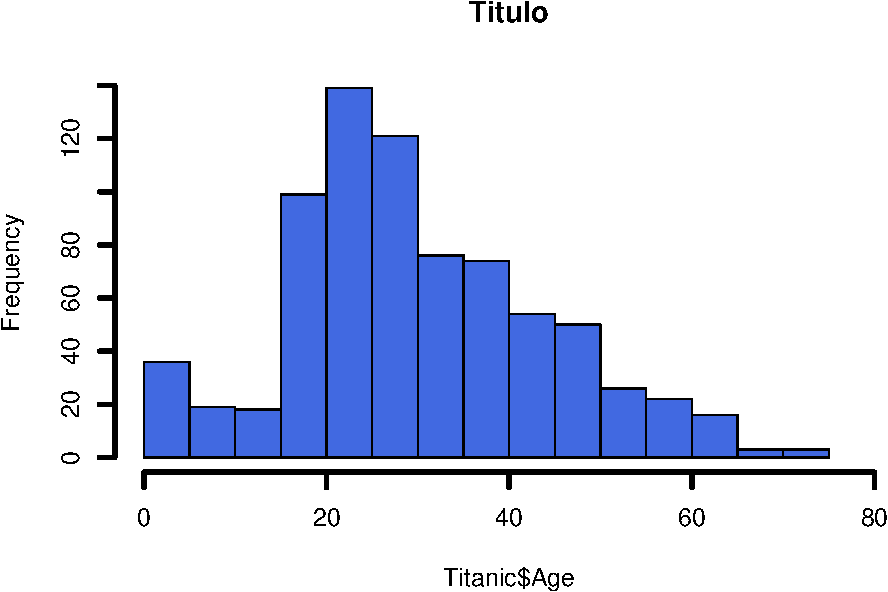
\includegraphics{intro-R_files/figure-latex/unnamed-chunk-113-1.pdf}

Para as variáveis categóricas geramos gráficos de barras com a função \texttt{barplot()} a partir da tabela de frequências da variável:

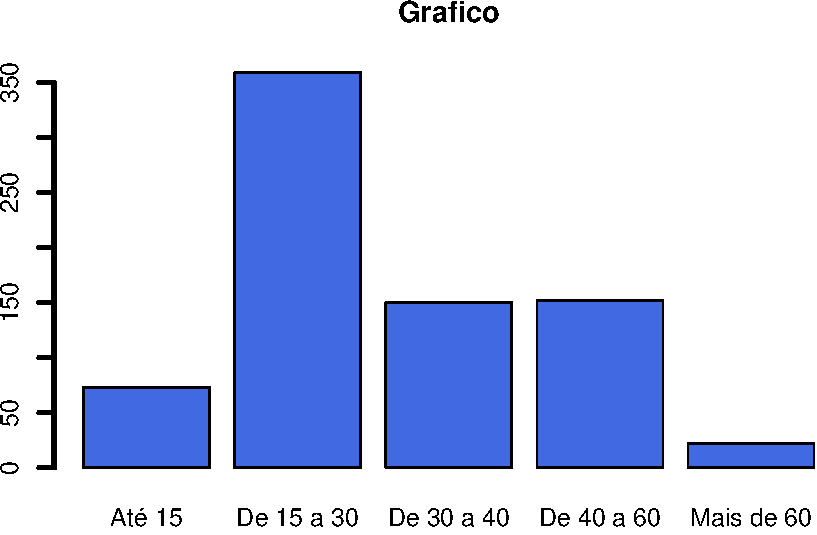
\includegraphics{intro-R_files/figure-latex/unnamed-chunk-114-1.pdf}

A função \texttt{boxplot()} possibilita a criação de boxplots. Podemos rotacionar os gráficos com o argumento \texttt{horizontal\ =\ TRUE}:

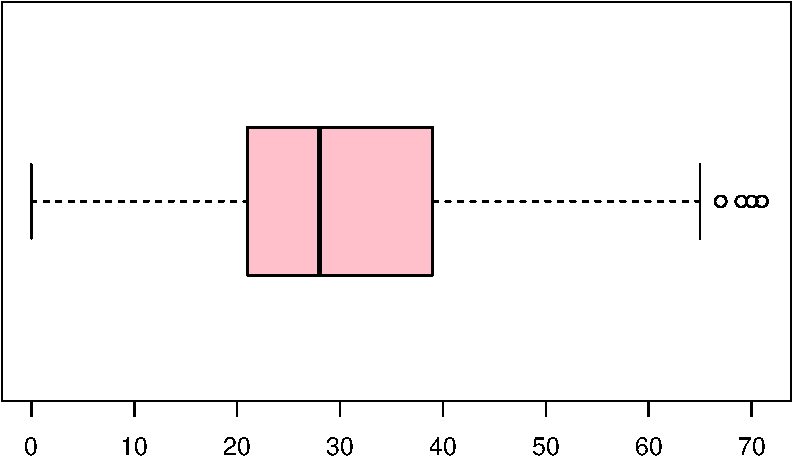
\includegraphics{intro-R_files/figure-latex/unnamed-chunk-115-1.pdf}

Podemos também realizar gráficos com duas variáveis categóricas combinadas. Com os argumentos \texttt{xlab} e \texttt{ylab} adicionamos os nomes dos eixos \texttt{x} e \texttt{y}:

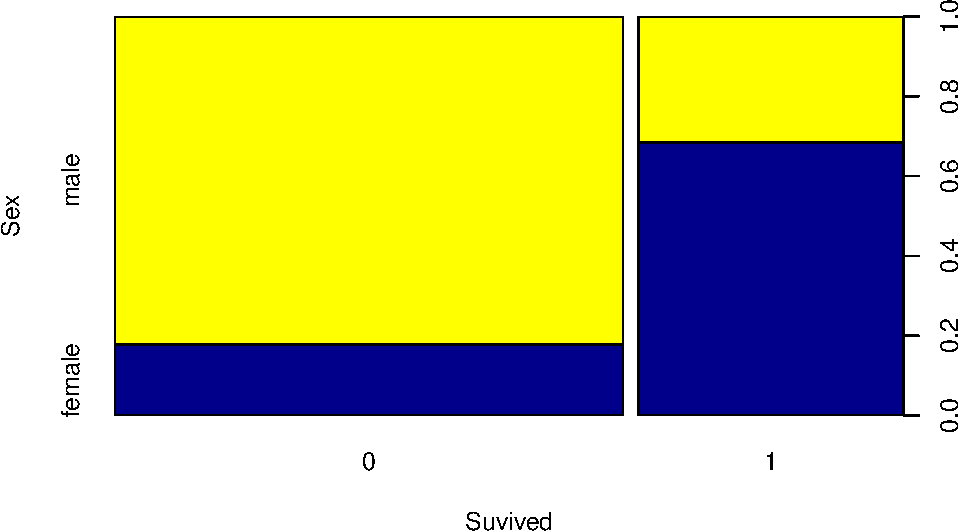
\includegraphics{intro-R_files/figure-latex/unnamed-chunk-116-1.pdf}

A partir da frequência da variável \texttt{PClass} que atribuímos anteriormente podemos realizar um gráfico de pizza, com a função \texttt{pie()}:

\begin{Shaded}
\begin{Highlighting}[]
\KeywordTok{pie}\NormalTok{(freq_class, }\DataTypeTok{main =} \StringTok{"Frequência das variável PClass"}\NormalTok{)}
\end{Highlighting}
\end{Shaded}

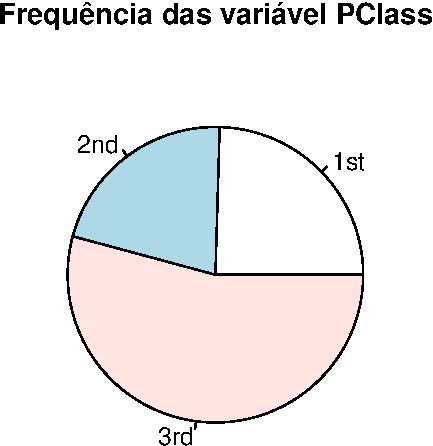
\includegraphics{intro-R_files/figure-latex/unnamed-chunk-117-1.pdf}

A partir da tabela de contigência das variáveis \texttt{Sex} e \texttt{Survived} podemos criar o gráfico de barras empilhadas. Adicionamos ainda a função \texttt{legend()} para adicionar a legenda das cores da variável \texttt{Sex}. Com o argumento da legenda \texttt{horiz\ =\ TRUE} dizemos que queremos que a legenda esteja na horizontal (uma categoria ao lado da outra), o argumento \texttt{pch} informa o código do símbolo que desejamos utilizar na legenda\footnote{Add Points to a Plot: \url{https://www.rdocumentation.org/packages/graphics/versions/3.6.1/topics/points}}, \texttt{inset} informa onde queremos colocar a legenda em relação a margem e \texttt{bty} como queremos a caixa da legenda (no caso deixamos a caixa sem borda e sem preenchimento). Ainda, a localização da legenda pode ser: \texttt{bottomright}, \texttt{bottom}, \texttt{bottomleft}, \texttt{left}, \texttt{topleft}, \texttt{top}, \texttt{topright}, \texttt{right} ou \texttt{center}.

\begin{Shaded}
\begin{Highlighting}[]
\KeywordTok{barplot}\NormalTok{(}\KeywordTok{table}\NormalTok{(Titanic}\OperatorTok{$}\NormalTok{Sex, Titanic}\OperatorTok{$}\NormalTok{Survived), }\DataTypeTok{ylim =} \KeywordTok{c}\NormalTok{(}\DecValTok{0}\NormalTok{,}\DecValTok{1000}\NormalTok{), }\DataTypeTok{xlab =} \StringTok{"Survived"}\NormalTok{, }\DataTypeTok{main =} \StringTok{"Distribuição"}\NormalTok{, }\DataTypeTok{col=}\KeywordTok{c}\NormalTok{(}\StringTok{"darkblue"}\NormalTok{, }\StringTok{"red"}\NormalTok{)) }
\KeywordTok{legend}\NormalTok{(}\StringTok{"top"}\NormalTok{, }\KeywordTok{c}\NormalTok{(}\StringTok{"Female"}\NormalTok{, }\StringTok{"Male"}\NormalTok{), }\DataTypeTok{horiz =} \OtherTok{TRUE}\NormalTok{, }\DataTypeTok{col =} \KeywordTok{c}\NormalTok{(}\StringTok{"darkblue"}\NormalTok{, }\StringTok{"red"}\NormalTok{), }\DataTypeTok{pch =} \DecValTok{16}\NormalTok{, }\DataTypeTok{inset =} \KeywordTok{c}\NormalTok{(}\DecValTok{0}\NormalTok{,}\DecValTok{0}\NormalTok{), }\DataTypeTok{bty =} \StringTok{"n"}\NormalTok{)}
\end{Highlighting}
\end{Shaded}

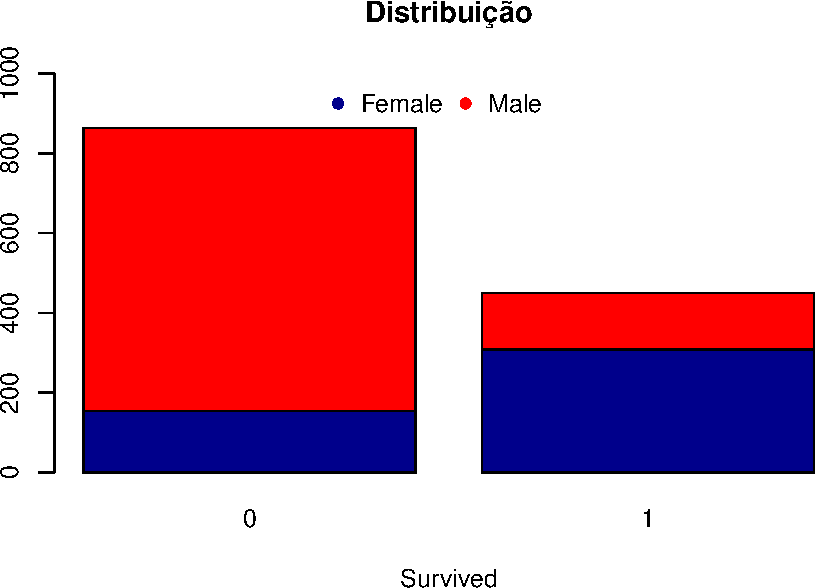
\includegraphics{intro-R_files/figure-latex/unnamed-chunk-118-1.pdf}

Por fim, podemos combinar diversos gráfico em uma mesma imagem. Para isso precisamos primeiro utilizar a função \texttt{par}, com o argumento \texttt{mfrow} informando a quantidade de linhas e colunas que queremos adicionar na nossa imagem. Aqui utilizaremos 1 linha com 2 colunas pois queremos 2 gráficos um do lado do outro. E o argumento \texttt{oma} informa o tamanho das margens externas da figura na ordem inferior, esquerda, superior e direita. Depois, nas linhas abaixo inserimos os gráficos desejados:

\begin{Shaded}
\begin{Highlighting}[]
\KeywordTok{par}\NormalTok{(}\DataTypeTok{mfrow =} \KeywordTok{c}\NormalTok{(}\DecValTok{1}\NormalTok{,}\DecValTok{2}\NormalTok{), }\DataTypeTok{oma =} \KeywordTok{c}\NormalTok{(}\DecValTok{1}\NormalTok{,}\DecValTok{1}\NormalTok{,}\DecValTok{1}\NormalTok{,}\DecValTok{1}\NormalTok{))}
\KeywordTok{plot}\NormalTok{(Titanic}\OperatorTok{$}\NormalTok{Survived, Titanic}\OperatorTok{$}\NormalTok{Sex, }\DataTypeTok{col =} \KeywordTok{c}\NormalTok{(}\StringTok{"Dark Blue"}\NormalTok{, }\StringTok{"Yellow"}\NormalTok{))}
\KeywordTok{plot}\NormalTok{(Titanic}\OperatorTok{$}\NormalTok{Survived, Titanic}\OperatorTok{$}\NormalTok{PClass, }\DataTypeTok{col =} \KeywordTok{c}\NormalTok{(}\StringTok{"Gray"}\NormalTok{, }\StringTok{"Dark Blue"}\NormalTok{, }\StringTok{"Red"}\NormalTok{))}
\end{Highlighting}
\end{Shaded}

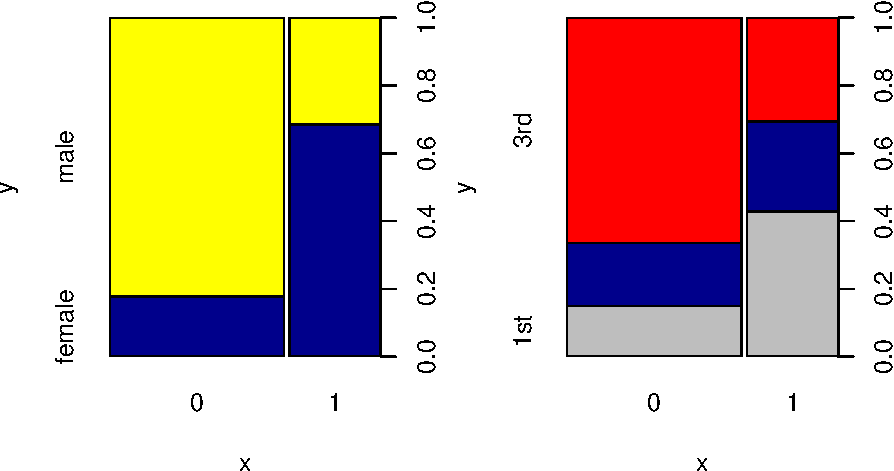
\includegraphics{intro-R_files/figure-latex/unnamed-chunk-119-1.pdf}

\hypertarget{impor}{%
\section{Importação e exportação de bancos de dados}\label{impor}}

Os bancos de dados disponibilizados no R são muito úteis mas também precisamos importar nossos bancos de dados para análise. O R possui diversas funcionalidades para importação dos mais diversos tipos de bancos de dados (.csv, .xlsx, .sav, etc). Aqui iremos ver como importar e exportar bancos \texttt{.csv}.

Para tanto precisamos utilizar as funções \texttt{read.csv()} para importar e \texttt{write.csv()} para exportar. O formato padrão de importação é:
read.csv(``nomebanco.csv'', na.strings = "``, stringsAsFactors = FALSE, header = TRUE, encoding =''UTF-8")

Onde,

\begin{itemize}
\tightlist
\item
  \texttt{nomebanco} é o nome do arquivo que você deseja importar. Se o arquivo não está no diretório raiz do seu projeto, é necessário colocar todo o endereço (Atenção que no Windows é necessário inverter as barras do endereço). é necessário a extensão do arquivo.
\item
  \texttt{na.strings} é a indicação para o R de qual string ele deve ler como NA. Se você não sabe como está configurado o seu banco utilize "" neste argumento. Assim o R irá ler apenas os locais em branco como NA
\item
  \texttt{header} é a indicação de que o seu banco tem um cabeçalho. Assim, o R irá ler a primeira linha como nome das colunas. Se o seu banco não tem cabeçalho atribua \texttt{FALSE} a esse argumento
\item
  \texttt{encoding} é a indicação da codificação do seu banco. Geralmente no Brasil utilizamos o \texttt{UTF-8}
\end{itemize}

\begin{quote}
Atenção! Se o seu banco está comfigurado com \texttt{,} como padrão de separação para decimais dos números é necessário utilizar a função \texttt{read.csv2()}
\end{quote}

Para exportar um banco já trabalhado no R utilize o seguinte comando:

write.csv(banco, file = ``nomearquivo.csv'', na = ``NA'')

Onde,

\begin{itemize}
\tightlist
\item
  \texttt{banco} é o nome do banco no R que você deseja exportar
\item
  \texttt{file} é o nome do arquivo que você deseja criar. Será salvo automaticamente na pasta raiz do seu projeto a não ser que você indique um outro endereço. é necessário a extensão do arquivo.
\item
  \texttt{na} é a indicação de como estão os NAs no seu banco.
\end{itemize}

\begin{quote}
Atenção! Se você deseja que seu banco seja salvo no padrão de seperação de decimais com \texttt{,} é necessário utilizar a função \texttt{write.csv2()}
\end{quote}

\hypertarget{tidy}{%
\chapter{Introdução ao Tidyverse}\label{tidy}}

Os pacotes \texttt{tidyverse} são uma coleção de pacotes criados por Hadley Wickham e sua equipe (na RStudio)\footnote{Tidy Data: \url{https://vita.had.co.nz/papers/tidy-data.html}} para facilitar o tratamento e visualização dos dados. Aqui, iremos ver alguns desses pacotes nos próximos capítulos. Para darmos início aos pacotes \texttt{tidyverse} precisamos instalá-los. Para instalar todos os pacotes do \texttt{tidyverse} utilize o comando \texttt{install.packages("tidyverse")} ou apenas os pacotes desejados. Aqui iremos utilizar os pacotes \texttt{tidyr}, \texttt{dplyr}, \texttt{stringr} e \texttt{lubridate}. Depois de instalados chame os pacotes com a função \texttt{library()}.

Antes de começarmos vamos só entender o que os criadores do \texttt{tidyverse} consideram como \texttt{tidydata}. A ideia de um banco de dados ``tidy'' é um banco de dados que tem:

1 - Cada variável forma uma coluna;
2 - Cada observação forma uma linha;
3 - Cada tipo de observação forma uma tabela (ou banco de dados)

Parece um pouco óbvio isso, mas certamente você já viu bancos de dados assim:

\begin{longtable}[]{@{}ccccc@{}}
\toprule
Nome & Preto & Amarelo & Castanho & Outro\tabularnewline
\midrule
\endhead
Joao & 0 & 1 & 0 & 0\tabularnewline
Luiz & 1 & 0 & 0 & 0\tabularnewline
Fabiana & 0 & 0 & 1 & 0\tabularnewline
Marcela & 1 & 0 & 0 & 0\tabularnewline
\bottomrule
\end{longtable}

Esse mesmo banco em um formato \texttt{tidy} ficaria:

\begin{longtable}[]{@{}cc@{}}
\toprule
Nome & Cor de cabelo\tabularnewline
\midrule
\endhead
Joao & Amarelo\tabularnewline
Luiz & Preto\tabularnewline
Fabiana & Castanho\tabularnewline
Marcela & Preto\tabularnewline
\bottomrule
\end{longtable}

Aqui iremos apresentar algumas das ferramentas dos pacotes do \texttt{tidyverse} para transformar os bancos em \texttt{tidydata}.

Primeiramente, iremos utilizar o banco \href{https://raw.githubusercontent.com/ipassos/material-introR/master/banco.csv}{Países}. Salve o arquivo \texttt{.csv} em seu computador e importe-o para o R sem considerar strings como factors e lendo as cédulas em branco como NA (no subcapítulo \ref{impor} há algumas instruções para importação de banco de dados).

Após importar o banco \texttt{Países} veja a estrutura e o resumo do banco.

\begin{Shaded}
\begin{Highlighting}[]
\KeywordTok{summary}\NormalTok{(paises)}
\end{Highlighting}
\end{Shaded}

\begin{verbatim}
##      pais              codigo           continente            X1970      
##  Length:249         Length:249         Length:249         Min.   :201.0  
##  Class :character   Class :character   Class :character   1st Qu.:354.0  
##  Mode  :character   Mode  :character   Mode  :character   Median :501.0  
##                                                           Mean   :508.1  
##                                                           3rd Qu.:668.0  
##                                                           Max.   :794.0  
##                                                                          
##      X1971           X1972           X1973         X1974      
##  Min.   :200.0   Min.   :200.0   Min.   :202   Min.   :201.0  
##  1st Qu.:325.0   1st Qu.:350.0   1st Qu.:396   1st Qu.:338.5  
##  Median :505.0   Median :495.0   Median :544   Median :481.0  
##  Mean   :495.2   Mean   :496.7   Mean   :529   Mean   :495.9  
##  3rd Qu.:642.0   3rd Qu.:644.0   3rd Qu.:658   3rd Qu.:656.5  
##  Max.   :798.0   Max.   :800.0   Max.   :799   Max.   :800.0  
##  NA's   :4                       NA's   :4     NA's   :1      
##      X1975           X1976           X1977           X1978      
##  Min.   :202.0   Min.   :200.0   Min.   :202.0   Min.   :200.0  
##  1st Qu.:358.0   1st Qu.:339.0   1st Qu.:360.0   1st Qu.:338.0  
##  Median :501.0   Median :512.0   Median :503.0   Median :492.0  
##  Mean   :495.4   Mean   :497.5   Mean   :505.5   Mean   :491.5  
##  3rd Qu.:631.5   3rd Qu.:641.0   3rd Qu.:667.0   3rd Qu.:637.0  
##  Max.   :798.0   Max.   :796.0   Max.   :791.0   Max.   :800.0  
##  NA's   :1                       NA's   :4       NA's   :2      
##      X1979           X1980           X1981            X1982      
##  Min.   :201.0   Min.   :207.0   Min.   : 200.0   Min.   :204.0  
##  1st Qu.:335.8   1st Qu.:384.5   1st Qu.: 365.0   1st Qu.:369.0  
##  Median :492.5   Median :530.0   Median : 509.0   Median :508.0  
##  Mean   :487.6   Mean   :514.3   Mean   : 531.3   Mean   :511.5  
##  3rd Qu.:626.8   3rd Qu.:645.0   3rd Qu.: 629.0   3rd Qu.:671.0  
##  Max.   :789.0   Max.   :799.0   Max.   :7520.0   Max.   :800.0  
##  NA's   :1       NA's   :1       NA's   :2                       
##      X1983           X1984            X1985           X1986       
##  Min.   :201.0   Min.   : 200.0   Min.   :202.0   Min.   : 200.0  
##  1st Qu.:354.0   1st Qu.: 345.0   1st Qu.:383.0   1st Qu.: 374.5  
##  Median :487.0   Median : 490.0   Median :515.0   Median : 514.5  
##  Mean   :494.8   Mean   : 519.5   Mean   :518.7   Mean   : 531.6  
##  3rd Qu.:648.0   3rd Qu.: 651.0   3rd Qu.:674.0   3rd Qu.: 659.5  
##  Max.   :800.0   Max.   :7000.0   Max.   :800.0   Max.   :5150.0  
##                                                   NA's   :3       
##      X1987           X1988            X1989           X1990      
##  Min.   :200.0   Min.   : 200.0   Min.   :200.0   Min.   :201.0  
##  1st Qu.:357.5   1st Qu.: 346.0   1st Qu.:351.2   1st Qu.:351.0  
##  Median :485.0   Median : 498.0   Median :510.0   Median :501.5  
##  Mean   :499.7   Mean   : 528.9   Mean   :508.4   Mean   :498.1  
##  3rd Qu.:641.5   3rd Qu.: 656.2   3rd Qu.:680.5   3rd Qu.:635.8  
##  Max.   :798.0   Max.   :7550.0   Max.   :800.0   Max.   :800.0  
##  NA's   :2       NA's   :1        NA's   :1       NA's   :1      
##      X1991           X1992           X1993           X1994      
##  Min.   :202.0   Min.   :203.0   Min.   :201.0   Min.   :200.0  
##  1st Qu.:356.5   1st Qu.:351.0   1st Qu.:364.5   1st Qu.:353.0  
##  Median :520.5   Median :481.0   Median :518.0   Median :494.0  
##  Mean   :512.2   Mean   :494.6   Mean   :507.3   Mean   :506.6  
##  3rd Qu.:666.0   3rd Qu.:646.0   3rd Qu.:648.2   3rd Qu.:666.0  
##  Max.   :794.0   Max.   :799.0   Max.   :800.0   Max.   :800.0  
##  NA's   :3                       NA's   :1                      
##      X1995           X1996           X1997         X1998      
##  Min.   :203.0   Min.   :201.0   Min.   :200   Min.   :203.0  
##  1st Qu.:372.0   1st Qu.:338.0   1st Qu.:345   1st Qu.:335.5  
##  Median :530.0   Median :470.0   Median :492   Median :508.0  
##  Mean   :518.3   Mean   :484.1   Mean   :502   Mean   :503.3  
##  3rd Qu.:668.0   3rd Qu.:627.0   3rd Qu.:669   3rd Qu.:673.0  
##  Max.   :800.0   Max.   :799.0   Max.   :800   Max.   :799.0  
##  NA's   :4       NA's   :1                     NA's   :2      
##      X1999           X2000           date          
##  Min.   :200.0   Min.   :201.0   Length:249        
##  1st Qu.:356.5   1st Qu.:358.0   Class :character  
##  Median :504.5   Median :476.0   Mode  :character  
##  Mean   :505.0   Mean   :495.7                     
##  3rd Qu.:664.2   3rd Qu.:634.0                     
##  Max.   :797.0   Max.   :799.0                     
##  NA's   :3
\end{verbatim}

\hypertarget{verificauxe7uxe3o-de-nas}{%
\section{Verificação de NAs}\label{verificauxe7uxe3o-de-nas}}

Primeiro iremos verificar se o R identificou se há \texttt{missings} (NAs) no nosso banco (lembre-se que importamos as cédulas em branco como NAs). Para isso iremos utilizar 3 funções. A função \texttt{is.na()} retorna \texttt{TRUE} (quando não é NA) e \texttt{FALSE} (quando é NA) para todos elementos do banco. Não é muito útil, mas poderemos utilizá-la combinada com outras funções. Combinando com a função \texttt{any()} descobrimos se há algum NA no nosso banco:

\begin{Shaded}
\begin{Highlighting}[]
\KeywordTok{any}\NormalTok{(}\KeywordTok{is.na}\NormalTok{(paises))}
\end{Highlighting}
\end{Shaded}

\begin{verbatim}
## [1] TRUE
\end{verbatim}

Mas seria melhor se tivéssemos mais informações. Combinando \texttt{is.na()} com a função \texttt{sum()} descobrimos quantos NAs temos no nosso banco:

\begin{Shaded}
\begin{Highlighting}[]
\KeywordTok{sum}\NormalTok{(}\KeywordTok{is.na}\NormalTok{(paises))}
\end{Highlighting}
\end{Shaded}

\begin{verbatim}
## [1] 42
\end{verbatim}

\hypertarget{criando-tidydata-com-o-pacote-tidyr}{%
\section{Criando tidydata com o pacote tidyr}\label{criando-tidydata-com-o-pacote-tidyr}}

O nosso banco países tem um grande problema: temos diversas variáveis com nomes de anos fazendo com que o nosso banco tenha muitas variáveis. Lembrando do exemplo do começo do capítulo o certo seria termos uma variável \texttt{ano} com o número do ano correspondente e uma varíavel \texttt{valor} com o valor correspondente do ano. Isso faria com que a quantidade de linhas do nosso banco seja multiplicada por 30 pois iremos repetir cada país 30 vezes (uma para cada ano).

Poderíamos fazer essa alteração na mão utilizando editores de planilhas ou, com linguagens de programação, usando laços lógicos e de repetição. Por sorte, o pacote \texttt{tidyr} nos ajuda nesse sentido. A função \texttt{gather()} faz exatamente o que queremos. O primeiro argumento da função \texttt{gather} é o banco que iremos transformar. Depois, o nome da coluna em que juntaremos todas as outras (as 30 colunas com informações dos anos, no nosso caso) e o nome da coluna que tem os valores correspondentes da coluna anterior (no caso criamos a coluna \texttt{valor}). Por fim, informamos quais são as colunas que não irão sofrer alteração com a seguinte sintaxe: \texttt{-c(coluna1,\ coluna2)}. A seguir fazemos a transformação atribuindo ao banco \texttt{pais\_tidy}:

\begin{Shaded}
\begin{Highlighting}[]
\NormalTok{pais_tidy <-}\StringTok{ }\KeywordTok{gather}\NormalTok{(paises, ano, valor, }\OperatorTok{-}\KeywordTok{c}\NormalTok{(pais, codigo, continente, date))}
\end{Highlighting}
\end{Shaded}

Veja como o nosso banco \texttt{pais\_tidy} ficou:

\begin{Shaded}
\begin{Highlighting}[]
\KeywordTok{summary}\NormalTok{(pais_tidy)}
\end{Highlighting}
\end{Shaded}

\begin{verbatim}
##      pais              codigo           continente       
##  Length:7719        Length:7719        Length:7719       
##  Class :character   Class :character   Class :character  
##  Mode  :character   Mode  :character   Mode  :character  
##                                                          
##                                                          
##                                                          
##                                                          
##      date               ano                valor       
##  Length:7719        Length:7719        Min.   : 200.0  
##  Class :character   Class :character   1st Qu.: 354.0  
##  Mode  :character   Mode  :character   Median : 503.0  
##                                        Mean   : 506.1  
##                                        3rd Qu.: 654.0  
##                                        Max.   :7550.0  
##                                        NA's   :42
\end{verbatim}

Agora temos um banco \texttt{tidy}. Veja a diferença entre as dimensões do banco \texttt{paises} e do banco \texttt{pais\_tidy}:

\begin{tabular}{l|l|l}
\hline
  & paises & pais\_tidy\\
\hline
n\_rows & 249 & 7719\\
\hline
n\_cols & 35 & 6\\
\hline
\end{tabular}

Bom, também podemos fazer o processo inverso de transformar o banco em um \texttt{tidydata}. No caso, revertiríamos ao que era originalmente o nosso banco \texttt{paises}. Para isso utilizamos a função \texttt{spread()}. Nela, informamos no primeiro argumento o banco que iremos retirar as nossas informações (no caso é o banco \texttt{pais\_tidy}). Depois informamos qual a colunas que iremos separar e várias colunas (\texttt{ano} no nosso caso) e a coluna que contem os valores dessa coluna (\texttt{valor} no nosso caso):

\begin{Shaded}
\begin{Highlighting}[]
\NormalTok{pais_wide <-}\StringTok{ }\KeywordTok{spread}\NormalTok{(pais_tidy, ano, valor)}
\end{Highlighting}
\end{Shaded}

Veja a primeira linha do nosso banco \texttt{pais\_wide}:

\begin{verbatim}
##                                                  pais codigo continente
## 1                                            Dominica    DM          NA
##       date X1970 X1971 X1972 X1973 X1974 X1975 X1976 X1977 X1978 X1979
## 1 23/05/17   769   501   597   212   307   258   529   550   206   280
##   X1980 X1981 X1982 X1983 X1984 X1985 X1986 X1987 X1988 X1989 X1990 X1991
## 1   221   578   503   686   374   416    NA   572   561   638   559   294
##   X1992 X1993 X1994 X1995 X1996 X1997 X1998 X1999 X2000
## 1   777   579   634   560   583   783   674   667   521
\end{verbatim}

Outras funcionalidades do \texttt{tidyr} é criar bancos unindo e separando colunas de um banco já existente. Por exemplo, se eu quero um banco que tenha as colunas \texttt{pais} e \texttt{codigo} do meu banco \texttt{paises} unidas em uma coluna só posso unir essas colunas utilizando a função \texttt{unite()}. Informo no primeiro argumento o nome do meu banco original, depois o nome da coluna nova (a união das colunas) e as colunas que quero unir na sequência desejada. Depois informo com qual símbolo devo separar as informações na nova coluna.

\begin{Shaded}
\begin{Highlighting}[]
\NormalTok{pais_unido <-}\StringTok{ }\KeywordTok{unite}\NormalTok{(paises, pais_cod, pais, codigo, }\DataTypeTok{sep =} \StringTok{"/"}\NormalTok{)}
\end{Highlighting}
\end{Shaded}

A primeira linha do meu banco:

\begin{verbatim}
##                           pais_cod continente X1970 X1971 X1972 X1973
## 1                  Afganistán/ AF          AS   335   263   366   757
##   X1974 X1975 X1976 X1977 X1978 X1979 X1980 X1981 X1982 X1983 X1984 X1985
## 1   603   266   571   336   480   402   552   526   228   463   211   593
##   X1986 X1987 X1988 X1989 X1990 X1991 X1992 X1993 X1994 X1995 X1996 X1997
## 1   568   346   495   341   212   399   364   333   340   460   374   674
##   X1998 X1999 X2000     date
## 1   490   665   443 07/09/14
\end{verbatim}

Para fazer o processo contrário da função \texttt{unite()} utilizo a função \texttt{separate()}. Primeiro informo qual banco será separado, depois o nome da coluna a ser separada (argumento \texttt{col\ =}), depois o nome das colunas a serem criadas no argumento \texttt{into\ =\ c()} e o caracter na qual a função irá separar a coluna no argumento \texttt{sep\ =} (no caso é o símbolo \texttt{/}):

\begin{Shaded}
\begin{Highlighting}[]
\NormalTok{pais_sep <-}\StringTok{ }\KeywordTok{separate}\NormalTok{(pais_unido, }\DataTypeTok{col =}\NormalTok{ pais_cod, }\DataTypeTok{into =} \KeywordTok{c}\NormalTok{(}\StringTok{"pais"}\NormalTok{, }\StringTok{"cod"}\NormalTok{), }\DataTypeTok{sep =} \StringTok{"/"}\NormalTok{)}
\end{Highlighting}
\end{Shaded}

A primeira linha do nosso banco:

\begin{verbatim}
##                          pais  cod continente X1970 X1971 X1972 X1973
## 1                  Afganistán  AF          AS   335   263   366   757
##   X1974 X1975 X1976 X1977 X1978 X1979 X1980 X1981 X1982 X1983 X1984 X1985
## 1   603   266   571   336   480   402   552   526   228   463   211   593
##   X1986 X1987 X1988 X1989 X1990 X1991 X1992 X1993 X1994 X1995 X1996 X1997
## 1   568   346   495   341   212   399   364   333   340   460   374   674
##   X1998 X1999 X2000     date
## 1   490   665   443 07/09/14
\end{verbatim}

\hypertarget{manipulauxe7uxe3o-de-strings}{%
\section{Manipulação de strings}\label{manipulauxe7uxe3o-de-strings}}

O pacote \texttt{stringr} tem várias ferramentas para nos ajudar na manipulação de strings. O nosso banco \texttt{paises} veio com vários erros na coluna \texttt{pais}. Alguns nomes de países tem espaços antes e/ou depois do nome do país. A função \texttt{str\_trim()} ajuda a retirar esses espaços de forma automatizada. Atribuímos o resultado da função ao próprio banco.

\begin{quote}
Preste muita atenção ao realizar funções sobrescrevendo o banco original
\end{quote}

\begin{Shaded}
\begin{Highlighting}[]
\NormalTok{pais_tidy}\OperatorTok{$}\NormalTok{pais <-}\StringTok{ }\KeywordTok{str_trim}\NormalTok{(pais_tidy}\OperatorTok{$}\NormalTok{pais)}
\end{Highlighting}
\end{Shaded}

Veja que a função limpou os nomes dos países no banco \texttt{pais\_tidy}.

\BeginKnitrBlock{exercise}
\protect\hypertarget{exr:unnamed-chunk-135}{}{\label{exr:unnamed-chunk-135} }Realize a limpeza dos nomes nos outros bancos criados a partir do banco \texttt{paises}.
\EndKnitrBlock{exercise}

Uma outra função útil é a \texttt{str\_pad()}, que adiciona strings a uma coluna de um banco de dados. Por exemplo, se quisermos adicionar o caracter \texttt{X} depois das siglas do continente na coluna \texttt{continente} do banco \texttt{pais\_unido}. Atribuímos a coluna do banco desejado a função \texttt{str\_pad()} com o primeiro argumento a referência da coluna desejada, depois no argumento \texttt{width\ =} informamos qual vai ser o tamanho dessa nova \texttt{string} (no caso as siglas já tinham o tamanho 2, com a adição de um novo caracter era irá passar a ter tamanho 3), o argumento \texttt{side\ =} informa onde a string irá (left ou right) e o argumento \texttt{pad\ =} informa qual a sequência de caracteres que iremos adicionar:

\begin{Shaded}
\begin{Highlighting}[]
\NormalTok{pais_unido}\OperatorTok{$}\NormalTok{continente <-}\StringTok{ }\KeywordTok{str_pad}\NormalTok{(pais_unido}\OperatorTok{$}\NormalTok{continente, }\DataTypeTok{width =} \DecValTok{3}\NormalTok{, }\DataTypeTok{side =} \StringTok{"right"}\NormalTok{, }\DataTypeTok{pad =} \StringTok{"X"}\NormalTok{)}
\end{Highlighting}
\end{Shaded}

Resultando em:

\begin{verbatim}
##                           pais_cod continente X1970 X1971 X1972 X1973
## 1                  Afganistán/ AF         ASX   335   263   366   757
## 2  Albania                   / AL         EUX   516   270   403   450
##   X1974 X1975 X1976 X1977 X1978 X1979 X1980 X1981 X1982 X1983 X1984 X1985
## 1   603   266   571   336   480   402   552   526   228   463   211   593
## 2   236   314   668   412   549   468   729   297   706   729   401   364
##   X1986 X1987 X1988 X1989 X1990 X1991 X1992 X1993 X1994 X1995 X1996 X1997
## 1   568   346   495   341   212   399   364   333   340   460   374   674
## 2   263   628   709   729   352   506   253   705   278   515   645   689
##   X1998 X1999 X2000     date
## 1   490   665   443 07/09/14
## 2   676   439   795 08/09/14
\end{verbatim}

Outra funcionalidade é detectar onde em um banco uma série de caracteres se encontra com a função \texttt{str\_detect()}:

\begin{Shaded}
\begin{Highlighting}[]
\KeywordTok{str_detect}\NormalTok{(pais_sep}\OperatorTok{$}\NormalTok{continente, }\StringTok{"NA"}\NormalTok{)}
\end{Highlighting}
\end{Shaded}

\begin{verbatim}
##   [1] FALSE FALSE FALSE FALSE FALSE  TRUE FALSE  TRUE FALSE FALSE FALSE
##  [12] FALSE  TRUE FALSE FALSE FALSE  TRUE FALSE  TRUE FALSE FALSE  TRUE
##  [23] FALSE  TRUE FALSE FALSE  TRUE FALSE FALSE FALSE FALSE FALSE FALSE
##  [34] FALSE FALSE FALSE FALSE FALSE  TRUE FALSE FALSE FALSE FALSE FALSE
##  [45] FALSE FALSE FALSE FALSE FALSE FALSE  TRUE FALSE  TRUE  TRUE FALSE
##  [56]  TRUE FALSE FALSE  TRUE FALSE FALSE FALSE FALSE FALSE  TRUE FALSE
##  [67] FALSE FALSE FALSE FALSE FALSE FALSE FALSE FALSE FALSE FALSE FALSE
##  [78]  TRUE FALSE  TRUE  TRUE FALSE  TRUE FALSE FALSE FALSE FALSE FALSE
##  [89] FALSE  TRUE  TRUE FALSE FALSE FALSE FALSE FALSE FALSE FALSE FALSE
## [100] FALSE FALSE FALSE FALSE FALSE  TRUE FALSE FALSE FALSE FALSE FALSE
## [111] FALSE FALSE FALSE FALSE  TRUE FALSE  TRUE  TRUE FALSE FALSE  TRUE
## [122] FALSE FALSE FALSE FALSE FALSE FALSE FALSE FALSE FALSE FALSE FALSE
## [133] FALSE FALSE FALSE FALSE FALSE FALSE FALSE FALSE FALSE FALSE FALSE
## [144] FALSE FALSE FALSE  TRUE FALSE FALSE FALSE  TRUE FALSE FALSE FALSE
## [155] FALSE FALSE  TRUE FALSE FALSE FALSE FALSE FALSE  TRUE FALSE FALSE
## [166] FALSE FALSE FALSE FALSE FALSE FALSE FALSE FALSE FALSE  TRUE FALSE
## [177] FALSE FALSE FALSE FALSE FALSE FALSE  TRUE FALSE FALSE FALSE FALSE
## [188] FALSE  TRUE FALSE FALSE FALSE FALSE FALSE FALSE  TRUE  TRUE FALSE
## [199]  TRUE  TRUE  TRUE FALSE  TRUE FALSE FALSE FALSE FALSE FALSE FALSE
## [210] FALSE  TRUE FALSE FALSE FALSE FALSE FALSE FALSE FALSE FALSE FALSE
## [221] FALSE FALSE FALSE FALSE FALSE FALSE FALSE FALSE FALSE FALSE FALSE
## [232] FALSE  TRUE FALSE FALSE FALSE FALSE FALSE FALSE FALSE FALSE FALSE
## [243] FALSE FALSE FALSE FALSE FALSE FALSE FALSE
\end{verbatim}

Podemos também substituir uma série de caracteres com a função \texttt{str\_replace()}. Por exemplo, substituíremos na coluna \texttt{continente} do banco \texttt{pais\_sep} todas os lugares que forem \texttt{NA} por \texttt{North\ America}:

\begin{Shaded}
\begin{Highlighting}[]
\NormalTok{pais_sep}\OperatorTok{$}\NormalTok{continente <-}\StringTok{ }\KeywordTok{str_replace}\NormalTok{(pais_sep}\OperatorTok{$}\NormalTok{continente, }\StringTok{"NA"}\NormalTok{, }\StringTok{"North America"}\NormalTok{)}
\end{Highlighting}
\end{Shaded}

Por fim, precisamos retirar da coluna \texttt{ano} em \texttt{pais\_tidy} a string \texttt{X} que foi herdada do nome das colunas de \texttt{pais}. Para isso utilizamos a função \texttt{str\_remove()}:

\begin{Shaded}
\begin{Highlighting}[]
\NormalTok{pais_tidy}\OperatorTok{$}\NormalTok{ano <-}\StringTok{ }\KeywordTok{str_remove}\NormalTok{(pais_tidy}\OperatorTok{$}\NormalTok{ano, }\StringTok{"X"}\NormalTok{)}
\end{Highlighting}
\end{Shaded}

\begin{quote}
A função \texttt{str\_remove} remove apenas o primeiro correspondente que ela encontra. Se a coluna tivesse mais de um ``X'' e quiséssemos remover todos os ``X'' da coluna deveríamos utilizar a função \texttt{str\_remove\_all()}.
\end{quote}

Por fim, nas funções \texttt{base} do R temos duas funções que nos são úteis para tratar com strings: \texttt{tolower()} e \texttt{toupper()}. A primeira faz com que todos os caracteres sejam transformados em caixa baixa e a segunda em caixa alta.

Veja a função \texttt{tolower()} na coluna \texttt{continente} do banco \texttt{pais\_wide}:

\begin{Shaded}
\begin{Highlighting}[]
\NormalTok{pais_wide}\OperatorTok{$}\NormalTok{continente <-}\StringTok{ }\KeywordTok{tolower}\NormalTok{(pais_wide}\OperatorTok{$}\NormalTok{continente) }
\KeywordTok{head}\NormalTok{(pais_wide)}
\end{Highlighting}
\end{Shaded}

\begin{verbatim}
##                                                  pais codigo continente
## 1                                            Dominica    DM          na
## 2                                        Burkina Faso    BF          af
## 3                                              Brasil    BR          sa
## 4                                           Guadalupe    GP          na
## 5                              Emiratos Árabes Unidos    AE          as
## 6                                          Afganistán    AF          as
##       date X1970 X1971 X1972 X1973 X1974 X1975 X1976 X1977 X1978 X1979
## 1 23/05/17   769   501   597   212   307   258   529   550   206   280
## 2 19/09/14   382   527   350   694   771   671   260   489   316   227
## 3 12/06/17   426   239   616   532   467   439   361   242   650   493
## 4 15/10/15   726   467   399   534   589   542   482   722   533   414
## 5 19/05/17   700   330   607   593   670   780   417   718   628   498
## 6 07/09/14   335   263   366   757   603   266   571   336   480   402
##   X1980 X1981 X1982 X1983 X1984 X1985 X1986 X1987 X1988 X1989 X1990 X1991
## 1   221   578   503   686   374   416    NA   572   561   638   559   294
## 2   234   612   754   735   599   661   771   319   291   208   471   385
## 3   615   286   273   661   781   654   425   776   317   582   464   288
## 4   435   224   572   745   239   242   657   684   429   463   520   367
## 5   662   462   752   212   374   677   651   720   676   333   591   566
## 6   552   526   228   463   211   593   568   346   495   341   212   399
##   X1992 X1993 X1994 X1995 X1996 X1997 X1998 X1999 X2000
## 1   777   579   634   560   583   783   674   667   521
## 2   623   513   730   764   413   480   247   507   488
## 3   583   538   537   456   784   694   774   343   356
## 4   471   672   718   651   475   788   534   522   391
## 5   612   315   529   699   296   471   215   745   365
## 6   364   333   340   460   374   674   490   665   443
\end{verbatim}

E a função \texttt{toupper()} na coluna \texttt{pais} do banco \texttt{pais\_sep}:

\begin{Shaded}
\begin{Highlighting}[]
\NormalTok{pais_sep}\OperatorTok{$}\NormalTok{pais <-}\StringTok{ }\KeywordTok{toupper}\NormalTok{(pais_sep}\OperatorTok{$}\NormalTok{pais)}
\KeywordTok{head}\NormalTok{(pais_sep)}
\end{Highlighting}
\end{Shaded}

\begin{verbatim}
##                           pais  cod    continente X1970 X1971 X1972 X1973
## 1                   AFGANISTÁN  AF             AS   335   263   366   757
## 2   ALBANIA                     AL             EU   516   270   403   450
## 3                     ALEMANIA  DE             EU   505   309   787   635
## 4                      ANDORRA  AD             EU   749   400   636   414
## 5                       ANGOLA  AO             AF   310    NA   399   594
## 6 ANGUILA                       AI  North America   348   254   613   621
##   X1974 X1975 X1976 X1977 X1978 X1979 X1980 X1981 X1982 X1983 X1984 X1985
## 1   603   266   571   336   480   402   552   526   228   463   211   593
## 2   236   314   668   412   549   468   729   297   706   729   401   364
## 3   566   298   748   657   263   612   464   605   736   387   764   278
## 4   264   556   766   362   645   427   600   258   516   355   410   375
## 5   273   441   519   597   794   436   553   592   791   255   763   551
## 6   481   254   645   388   279   589   579   800   502   389   359   434
##   X1986 X1987 X1988 X1989 X1990 X1991 X1992 X1993 X1994 X1995 X1996 X1997
## 1   568   346   495   341   212   399   364   333   340   460   374   674
## 2   263   628   709   729   352   506   253   705   278   515   645   689
## 3   253   359   389   714   339   707   631   648   780   637   286   311
## 4   681   218   203   222   676   251   671   784   796   225   439   460
## 5   770   399   422   235   223   622   502   491   458   292   741   249
## 6   428   389   768   580   782   792   770   511   670   672   364   216
##   X1998 X1999 X2000     date
## 1   490   665   443 07/09/14
## 2   676   439   795 08/09/14
## 3   769   533   787 09/09/14
## 4   795   446   256 10/09/14
## 5   269   399   526 11/09/14
## 6   260   461   477 12/09/14
\end{verbatim}

\hypertarget{identificando-erros-no-banco}{%
\section{Identificando erros no banco}\label{identificando-erros-no-banco}}

Alguns dos valores do nosso banco estão com erros (provavelmente por erro de digitação). Vamos dar uma olhada no \texttt{boxplot} da coluna valor:

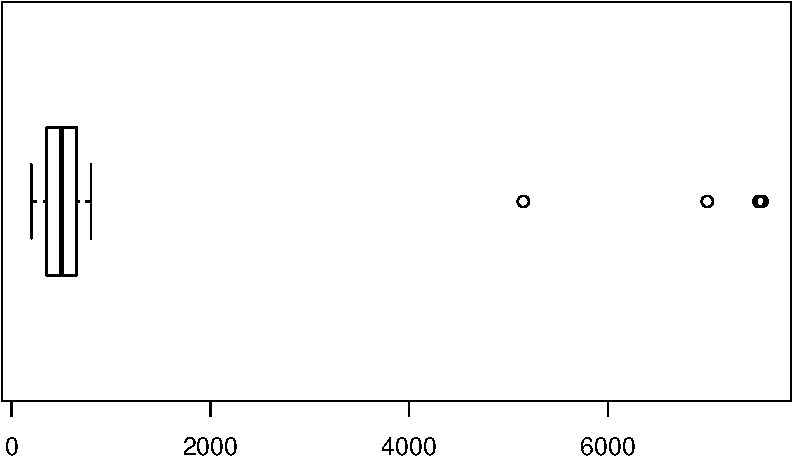
\includegraphics{intro-R_files/figure-latex/unnamed-chunk-143-1.pdf}

Os valores das colunas do banco \texttt{paises} foram gerados entre \texttt{200} e \texttt{800}. Portanto, a partir do boxplot podemos ver que há algo errado com o nosso banco. Vamos dar uma olhada no resumo das variáveis:

\begin{verbatim}
##    Min. 1st Qu.  Median    Mean 3rd Qu.    Max.    NA's 
##   200.0   354.0   503.0   506.1   654.0  7550.0      42
\end{verbatim}

\begin{quote}
O banco \texttt{paises} foi criado para ilustração dessa apostila. Ainda que pareça muito simples o exemplo podemos ter casos na realidade de situações em que idade de indivíduos, por exemplo, aparece como \texttt{200} no lugar de \texttt{20}.
\end{quote}

Vamos verificar quais são esses elementos:

\begin{Shaded}
\begin{Highlighting}[]
\KeywordTok{subset}\NormalTok{(pais_tidy, pais_tidy}\OperatorTok{$}\NormalTok{valor }\OperatorTok{>}\StringTok{ }\DecValTok{800}\NormalTok{)}
\end{Highlighting}
\end{Shaded}

\begin{verbatim}
##                                  pais codigo continente     date  ano
## 2751                          Armenia    AM          AS 14/06/17 1981
## 3512 Bolivia, Estado Plurinacional de    BO          SA 03/06/17 1984
## 4004                           Baréin    BH          AS 02/09/14 1986
## 4495                            Aruba    AW          NA 15/06/17 1988
##      valor
## 2751  7520
## 3512  7000
## 4004  5150
## 4495  7550
\end{verbatim}

Bom, pelo que podemos ver aparentemente foi um erro de digitação. Todos os casos tem um \texttt{0} a mais. Como estamos tratando de números e é simplesmente um \texttt{0} no final, vamos dividir todos os casos por \texttt{10}. Primeiro criamos um vetor com um endereço dos elementos que correspondem a busca (\texttt{pais\_tidy\$valor\ \textgreater{}\ 800}). Depois, substituímos esses valores por eles mesmos dividos por 10:

\begin{Shaded}
\begin{Highlighting}[]
\NormalTok{replace <-}\StringTok{ }\KeywordTok{which}\NormalTok{(pais_tidy}\OperatorTok{$}\NormalTok{valor }\OperatorTok{>}\StringTok{ }\DecValTok{800}\NormalTok{)}
\NormalTok{pais_tidy}\OperatorTok{$}\NormalTok{valor[}\KeywordTok{c}\NormalTok{(replace)] <-}\StringTok{ }\NormalTok{pais_tidy}\OperatorTok{$}\NormalTok{valor[}\KeywordTok{c}\NormalTok{(replace)]}\OperatorTok{/}\DecValTok{10}
\end{Highlighting}
\end{Shaded}

Vamos ver como eles ficaram?

\begin{Shaded}
\begin{Highlighting}[]
\NormalTok{pais_tidy[}\KeywordTok{c}\NormalTok{(replace), ]}
\end{Highlighting}
\end{Shaded}

\begin{verbatim}
##                                  pais codigo continente     date  ano
## 2751                          Armenia    AM          AS 14/06/17 1981
## 3512 Bolivia, Estado Plurinacional de    BO          SA 03/06/17 1984
## 4004                           Baréin    BH          AS 02/09/14 1986
## 4495                            Aruba    AW          NA 15/06/17 1988
##      valor
## 2751   752
## 3512   700
## 4004   515
## 4495   755
\end{verbatim}

E como será que o boxplot estará agora?

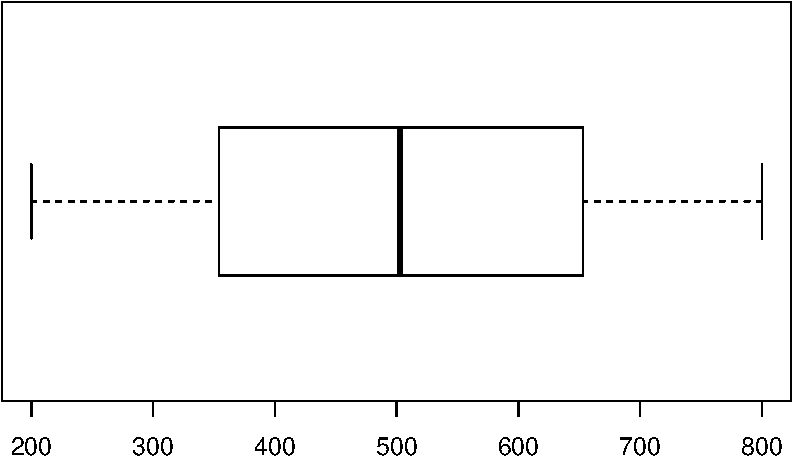
\includegraphics{intro-R_files/figure-latex/unnamed-chunk-148-1.pdf}

Pronto! Eliminamos todos os erros da variável \texttt{ano}.

\hypertarget{trabalhando-com-data-e-hora}{%
\section{Trabalhando com data e hora}\label{trabalhando-com-data-e-hora}}

O \texttt{tidyverse} também possui ótimas ferramentas para trabalharmos com datas e hora. O pacote \texttt{lubridate} agrega essas ferramentas. A coluna \texttt{date} do nosso banco \texttt{pais\_tidy} não está sendo lida pelo R como uma data, mas sim como um conjunto de caracteres:

\begin{Shaded}
\begin{Highlighting}[]
\KeywordTok{class}\NormalTok{(pais_tidy}\OperatorTok{$}\NormalTok{date)}
\end{Highlighting}
\end{Shaded}

\begin{verbatim}
## [1] "character"
\end{verbatim}

Bom, isso é um problema para análises futuras. Vamos então indicar para o R qual formato está a data do nosso banco. Se você der uma olhada no banco \texttt{pais\_tidy} verá que as datas estão da seguinte maneira: dd/mm/aa (em português). Para o R entender que isso é um formato de data precisamos indicar para ele. Assim, utilizamos as funções de formato de data do pacote \texttt{lubridate}. No caso, a função será \texttt{dmy} indicando que o formato é \texttt{day}, \texttt{month} e \texttt{year}:

\begin{Shaded}
\begin{Highlighting}[]
\NormalTok{pais_tidy}\OperatorTok{$}\NormalTok{date <-}\StringTok{ }\KeywordTok{dmy}\NormalTok{(pais_tidy}\OperatorTok{$}\NormalTok{date) }
\end{Highlighting}
\end{Shaded}

Veja agora como está a estrutura da nossa variável \texttt{date}:

\begin{Shaded}
\begin{Highlighting}[]
\KeywordTok{str}\NormalTok{(pais_tidy)}
\end{Highlighting}
\end{Shaded}

\begin{verbatim}
## 'data.frame':    7719 obs. of  6 variables:
##  $ pais      : chr  "Afganistán" "Albania" "Alemania" "Andorra" ...
##  $ codigo    : chr  " AF " " AL " " DE " " AD " ...
##  $ continente: chr  "AS" "EU" "EU" "EU" ...
##  $ date      : Date, format: "2014-09-07" "2014-09-08" ...
##  $ ano       : chr  "1970" "1970" "1970" "1970" ...
##  $ valor     : num  335 516 505 749 310 348 249 378 325 329 ...
\end{verbatim}

Agora as datas foram convertidas para o formato que o R entende como data:

\begin{Shaded}
\begin{Highlighting}[]
\KeywordTok{class}\NormalTok{(pais_tidy}\OperatorTok{$}\NormalTok{date)}
\end{Highlighting}
\end{Shaded}

\begin{verbatim}
## [1] "Date"
\end{verbatim}

Veja o resumo das nossas variáveis:

\begin{Shaded}
\begin{Highlighting}[]
\KeywordTok{summary}\NormalTok{(pais_tidy)}
\end{Highlighting}
\end{Shaded}

\begin{verbatim}
##      pais              codigo           continente       
##  Length:7719        Length:7719        Length:7719       
##  Class :character   Class :character   Class :character  
##  Mode  :character   Mode  :character   Mode  :character  
##                                                          
##                                                          
##                                                          
##                                                          
##       date                ano                valor      
##  Min.   :2014-08-05   Length:7719        Min.   :200.0  
##  1st Qu.:2014-10-06   Class :character   1st Qu.:354.0  
##  Median :2017-04-28   Mode  :character   Median :503.0  
##  Mean   :2016-05-21                      Mean   :502.9  
##  3rd Qu.:2017-06-29                      3rd Qu.:653.0  
##  Max.   :2018-05-08                      Max.   :800.0  
##                                          NA's   :42
\end{verbatim}

Podemos também informar outros formatos de datas. Utilizando a mesma função mas com a abreviação do mês:

\begin{Shaded}
\begin{Highlighting}[]
\KeywordTok{dmy}\NormalTok{(}\StringTok{"17 Nov 2015"}\NormalTok{)}
\end{Highlighting}
\end{Shaded}

\begin{verbatim}
## [1] "2015-11-17"
\end{verbatim}

Utilizando o formato com as horas, minutos e segundos:

\begin{Shaded}
\begin{Highlighting}[]
\KeywordTok{mdy_hms}\NormalTok{(}\StringTok{"July 15, 2012 12:56:09"}\NormalTok{)}
\end{Highlighting}
\end{Shaded}

\begin{verbatim}
## [1] "2012-07-15 12:56:09 UTC"
\end{verbatim}

\begin{quote}
Trabalhar com datas é bem mais complicado do que foi demonstrado aqui. Para mais informações veja o capítulo sobre datas e hora do livro \href{https://r4ds.had.co.nz/dates-and-times.html}{``R for Data Science''}
\end{quote}

\hypertarget{ajustes-finais}{%
\section{Ajustes finais}\label{ajustes-finais}}

Depois de todas essas alterações, para o nosso banco ficar pronto para análise vamos converter as variáveis \texttt{pais}, \texttt{codigo}, \texttt{continente} e \texttt{ano}. As três primeiras iremos transformar em \texttt{factor}:

\begin{Shaded}
\begin{Highlighting}[]
\NormalTok{pais_tidy}\OperatorTok{$}\NormalTok{pais <-}\StringTok{ }\KeywordTok{factor}\NormalTok{(pais_tidy}\OperatorTok{$}\NormalTok{pais)}
\NormalTok{pais_tidy}\OperatorTok{$}\NormalTok{codigo <-}\StringTok{ }\KeywordTok{factor}\NormalTok{(pais_tidy}\OperatorTok{$}\NormalTok{codigo)}
\NormalTok{pais_tidy}\OperatorTok{$}\NormalTok{continente <-}\StringTok{ }\KeywordTok{factor}\NormalTok{(pais_tidy}\OperatorTok{$}\NormalTok{continente)}
\end{Highlighting}
\end{Shaded}

Por fim, vamos criar uma variável \texttt{ano2} (cópia de \texttt{ano}) que será convertida em \texttt{factor} e vamos converter a variável \texttt{ano} em \texttt{numeric}:

\begin{Shaded}
\begin{Highlighting}[]
\NormalTok{pais_tidy}\OperatorTok{$}\NormalTok{ano2 <-}\StringTok{ }\NormalTok{pais_tidy}\OperatorTok{$}\NormalTok{ano}
\NormalTok{pais_tidy}\OperatorTok{$}\NormalTok{ano2 <-}\StringTok{ }\KeywordTok{factor}\NormalTok{(pais_tidy}\OperatorTok{$}\NormalTok{ano2)}
\NormalTok{pais_tidy}\OperatorTok{$}\NormalTok{ano <-}\StringTok{ }\KeywordTok{as.numeric}\NormalTok{(pais_tidy}\OperatorTok{$}\NormalTok{ano)}
\end{Highlighting}
\end{Shaded}

Agora o nosso banco estará assim:

\begin{verbatim}
##          pais          codigo     continente      date           
##  Afganistán:  31    AD    :  31   AF:1798    Min.   :2014-08-05  
##  Albania   :  31    AE    :  31   AN: 155    1st Qu.:2014-10-06  
##  Alemania  :  31    AF    :  31   AS:1643    Median :2017-04-28  
##  Andorra   :  31    AG    :  31   EU:1612    Mean   :2016-05-21  
##  Angola    :  31    AI    :  31   NA:1271    3rd Qu.:2017-06-29  
##  Anguila   :  31    AL    :  31   OC: 806    Max.   :2018-05-08  
##  (Other)   :7533   (Other):7533   SA: 434                        
##       ano           valor            ano2     
##  Min.   :1970   Min.   :200.0   1970   : 249  
##  1st Qu.:1977   1st Qu.:354.0   1971   : 249  
##  Median :1985   Median :503.0   1972   : 249  
##  Mean   :1985   Mean   :502.9   1973   : 249  
##  3rd Qu.:1993   3rd Qu.:653.0   1974   : 249  
##  Max.   :2000   Max.   :800.0   1975   : 249  
##                 NA's   :42      (Other):6225
\end{verbatim}

\hypertarget{ggplot}{%
\chapter{Gráficos com ggplot2}\label{ggplot}}

\hypertarget{mark}{%
\chapter{Relatórios com Markdown}\label{mark}}

\bibliography{book.bib,packages.bib}


\end{document}
